% ============================================================
%  RESS submission — full article
%  Compile: pdflatex main; bibtex main; pdflatex main; pdflatex main
%  Bibliography: reference.bib (existing) + new_bib_entries.bib
% ============================================================
\documentclass[review]{elsarticle}

\usepackage{amsmath, amssymb}
\usepackage{graphicx}
\usepackage{booktabs, multirow}
\usepackage{colortbl, xcolor}
\usepackage{algorithm}
\usepackage{algpseudocode}
\usepackage{rotating}
\usepackage[hidelinks]{hyperref}

\journal{Reliability Engineering \& System Safety}

\begin{document}

\begin{frontmatter}

\title{Three-Stage Framework for Bearing Remaining Useful Life
Prediction: Conditional GAN Augmentation, Multi-task Learning, and
Conformal Prediction Intervals}

\author[ensta]{Fatima Khadija Benzine}
% \author[...]{Co-author}
\affiliation[ensta]{organization={IECPS Laboratory, \'Ecole Nationale
Sup\'erieure de Technologie Avanc\'ee (ENSTA)}, city={Algiers},
country={Algeria}}

% ============================================================
%  Front matter: title, abstract, highlights, keywords, Section 1
% ============================================================

\begin{abstract}
Remaining useful life (RUL) predictions support maintenance decisions
only if their uncertainty is reported reliably, and most reliably in
the near-failure regime where decisions are taken. That regime is also
the least represented in run-to-failure data, and the few available
run-to-failure units leave little data for calibrating uncertainty.
This paper proposes a three-stage framework for bearing RUL prediction
that addresses these constraints together. A stage-conditioned
Wasserstein GAN synthesises complete multivariate near-failure windows
for training (C1). A multi-task BiLSTM with temporal attention predicts
the RUL and the degradation stage jointly from a shared encoder (C2).
Stage-conditional cross-conformal prediction (CV+) turns each point
prediction into an interval, uses every non-test bearing for
calibration, and conditions the interval on the stage predicted by
C2 (C3). Stage labels and RUL targets are derived automatically from a
guarded health-indicator criterion. On the XJTU-SY dataset, evaluated
with bearing-level cross-validation over five seeds, multi-task
learning lowers the near-failure RMSE from 0.225 to 0.206 and the
overall RMSE from 0.385 to 0.291. Cross-conformal calibration restores
nominal coverage: 0.917 overall at a 90\% target, against 0.74--0.83
for split conformal calibrated on two bearings. Conditioning on the
stage predicted by the multi-task model narrows the intervals of the
full framework by about 20\% relative to a single quantile, at higher
coverage.
Generative augmentation produces realistic windows but does not change
accuracy or interval quality significantly on its own. A per-bearing
analysis shows that coverage holds on average over bearings but not
for every bearing, with the shortest-lived bearings least well
covered.
\end{abstract}

\begin{highlights}
\item Stage labels and piecewise RUL targets derived without manual annotation.
\item Multi-task RUL and stage learning lowers near-failure and overall RMSE.
\item Cross-conformal calibration uses all non-test bearings and restores 90\% coverage.
\item The predicted stage narrows conformal intervals by about 20\% at equal coverage.
\item Per-bearing coverage exposes the limits of the guarantee on short-lived bearings.
\end{highlights}

\begin{keyword}
Remaining useful life \sep Rolling bearings \sep Conformal prediction
\sep Uncertainty quantification \sep Multi-task learning
\sep Generative adversarial networks
\end{keyword}

\end{frontmatter}

% ------------------------------------------------------------
\section{Introduction}
\label{sec:introduction}

Rolling bearings are among the most frequent sources of failure in
rotating machinery, and their unplanned failure stops production and
can damage surrounding components. Predictive maintenance addresses
this by estimating the remaining useful life (RUL) of each bearing from
its condition-monitoring signals and scheduling intervention before
failure. Deep learning models trained on vibration data now estimate
bearing RUL with good average accuracy on public run-to-failure
benchmarks such as XJTU-SY~\cite{8576668, lei2019xjtusy}. A point
estimate alone, however, is a weak basis for a maintenance decision.
The decision maker must also know how far the true RUL may lie from the
estimate, and this knowledge matters most close to failure, when the
cost of an error is highest.\\

Three properties of run-to-failure data make this difficult. First,
bearings spend most of their life in a healthy state, so the
near-failure regime, where predictions matter most, is the least
represented in the training data. Second, most uncertainty estimates
used for RUL, such as Bayesian layers, Monte Carlo dropout or Gaussian
output layers, rest on distributional assumptions and carry no
coverage guarantee; they are frequently overconfident in
practice~\cite{wang_uncertainty-aware_2026}. Conformal
prediction~\cite{vovk2005algorithmic, lei2018distribution} removes
these assumptions and provides intervals with finite-sample coverage,
but its guarantee rests on the calibration data resembling the test
data. Third, a run-to-failure dataset contains few units: XJTU-SY has
fifteen bearings. Holding out a calibration set therefore leaves very
few bearings to represent the variability between units, and the
coverage guarantee, which is formally marginal, may not hold where it
is needed.\\

Each of these difficulties has been addressed separately. Generative
adversarial networks have been used to enlarge the near-failure
regime~\cite{9486650, lu_joint_2022}, mostly on scalar health
indicators and evaluated through point accuracy only. Multi-task
models that predict the degradation stage alongside the RUL improve the
learned representation~\cite{8709822}. Conformal prediction has very
recently been applied to bearing RUL~\cite{wang_uncertainty-aware_2026,
11373138}, with coverage reported in aggregate over all windows. No
existing study combines the three, and none conditions the conformal
interval on the degradation stage that a multi-task model predicts, or
addresses the small number of units available for calibration.\\

This paper proposes a three-stage framework that addresses these
constraints together, and makes the following contributions:
\begin{itemize}
  \item \textbf{C1, stage-conditioned generative augmentation.} A
  Wasserstein GAN with gradient penalty, conditioned on the degradation
  stage, synthesises complete multivariate near-failure windows, which
  enter the training data only.
  \item \textbf{C2, multi-task RUL and stage prediction.} A BiLSTM with
  temporal attention predicts the RUL and the degradation stage from a
  shared encoder. The stage labels are derived automatically from a
  guarded health-indicator criterion, and the RUL target is piecewise.
  \item \textbf{C3, stage-conditional cross-conformal prediction.}
  Cross-conformal calibration (CV+) uses every non-test bearing for
  calibration, and the interval is conditioned on the stage predicted
  by the multi-task model of C2, so that a single network supplies the
  RUL estimate, the stage and the interval.
\end{itemize}
The framework is evaluated on XJTU-SY with bearing-level
cross-validation, a $2 \times 2$ ablation of C1 and C2, five random
seeds, and a per-bearing analysis of coverage. The evaluation is
reported with its full protocol (RUL scale, target shape, scoring
window and aggregation), so that the results can be compared with the
literature without ambiguity.\\

The remainder of the paper is organised as follows.
Section~\ref{sec:related_work} reviews related work.
Section~\ref{sec:methodology} presents the framework.
Section~\ref{sec:experimental_setup} describes the dataset, the data
preparation and the evaluation protocol. Section~\ref{sec:results}
reports the results, Section~\ref{sec:discussion} discusses them and
their limitations, and Section~\ref{sec:conclusion} concludes.


\section{Related work}
\label{sec:related_work}

\subsection{Deep Learning for Remaining Useful Life Prediction}
\label{sec:dl_rul}

Remaining useful life prediction methods can generally be grouped
into two broad categories~\cite{shang_capsule_2024, bai_towards_2024}.
The first, model-based methods, relies on mathematical modeling of
the physical degradation process and system dynamics. These approaches
are grounded in physics-based reasoning and offer accurate
threshold-based failure prediction under well-understood conditions.
However, the growing complexity of modern rotating machinery has made
it increasingly difficult to formulate accurate degradation models,
especially when the underlying mechanisms are non-linear or not fully
observable~\cite{heimes_recurrent_2008}. Moreover, model-based methods
often lack flexibility in adapting to diverse fault types and
operational conditions~\cite{shang_capsule_2024}. The second category,
data-driven methods, bypass this difficulty by learning
degradation patterns directly from sensor data, requiring less
domain-specific expertise and enabling rapid deployment without full
knowledge of the physical system~\cite{datadriven,
heimes_recurrent_2008}. Their performance, however, is strongly
conditioned on the volume, quality, and representativeness of the
available training data, a dependency that becomes critical in
industrial prognostics where run-to-failure experiments are both costly
and time-consuming~\cite{s25144481, pan2025remaining}.\\

Within the data-driven paradigm, early efforts relied on shallow
machine learning algorithms such as Artificial Neural
Networks~\cite{KHATIR2020102554}, Support Vector
Machines~\cite{TRAN2012320}, Random Forests~\cite{7508982randomforest},
and Hidden Markov Models~\cite{articleHiddenmarkov} for RUL estimation.
While these methods yielded promising initial results, they often
struggled to effectively handle the noisy, high-dimensional, and
temporally dependent nature of industrial sensor data. To address
these limitations, deep learning techniques were introduced into
the RUL prediction field. Convolutional Neural Networks (CNNs) were
among the earliest adopted, exploiting sliding-window representations
for spatial feature extraction from multivariate time series. Despite
their effectiveness in capturing local patterns, CNNs struggle to
retain long-range temporal dependencies, which are essential for
modeling the sequential nature of degradation
monitoring~\cite{shang_capsule_2024, pan2025remaining}. Recurrent
Neural Networks (RNNs) addressed this limitation through feedback
loops and internal memory states~\cite{articleRNNRUL}, enabling them
to approximate non-linear temporal dynamics. However, traditional RNNs
suffer from vanishing gradient issues that impair their ability to
learn long-term dependencies which is a key requirement in RUL
estimation~\cite{heimes_recurrent_2008}. Long Short-Term Memory
(LSTM) networks were subsequently introduced and rapidly adopted
for RUL prediction tasks, preserving information over longer time
horizons through gated mechanisms~\cite{inproceedingsLSTM}. Standard
LSTM architectures, however, tend to prioritize information from the
later parts of the input sequence, potentially ignoring critical
early-stage degradation signals that are often informative for bearing
prognostics~\cite{bai_towards_2024}.\\

To capture degradation dynamics in both temporal directions,
Bidirectional LSTM (BiLSTM) networks have emerged as a particularly
effective architecture for RUL estimation.
Ghavidel et al.~\cite{ghavidel_remaining_2026} conducted a
comparative evaluation of CNN, GRU, Transformer, and BiLSTM
architectures on bearing vibration data, demonstrating that BiLSTM
achieves the highest accuracy by capturing dependencies in both
forward and backward temporal directions. This finding is consistent
with recent bearing-specific architectures:
Wan et al.~\cite{wan_robust_2026} proposed a CNN-BiLSTM-TCN hybrid
that integrates spatial feature extraction, bidirectional temporal
modeling, and long-range dependency capture for bearing RUL on the
PRONOSTIA dataset;
Deng et al.~\cite{DENG2026112193} developed a collaborative
domain-adaptation bidirectional temporal convolution network validated
across multiple operating conditions on the XJTU-SY and PHM~2012
datasets; and
Liu et al.~\cite{liu_deep_2026} proposed a BiLSTM with self-attention
and a Bayesian linear layer for cross-domain bearing RUL prediction on
XJTU-SY. More recent work has explored
hybrid architectures that integrate recurrent and Transformer
components. Jiang et al.~\cite{s26051578} combined an extended LSTM
(xLSTM) with multi-head attention for bearing RUL prediction on
XJTU-SY, while
Yuntian et al.~\cite{YONGXING2026104313} introduced a temporal
self-attention mechanism within a dual-branch transfer network on the
same dataset. The attention mechanism
allows the model to dynamically weight the importance of individual
time steps, focusing on the most informative portions of the
degradation trajectory rather than treating all observations
uniformly. Several comprehensive reviews confirm the effectiveness
of these architectural trends: Tang et al.~\cite{tang_deep_2025}
reviewed deep learning-based hybrid models for bearing RUL
forecasting and identified attention-augmented recurrent architectures
as the current state of the art, while
Palaniappan et al.~\cite{palaniappan_systematic_2026} systematically
examined AI-based approaches across multiple bearing benchmark datasets
and reached a similar conclusion regarding the superiority of hybrid
deep learning models.\\

Although these architectures are frequently evaluated on the XJTU-SY
benchmark, their reported errors are difficult to compare directly. A
survey of recent XJTU-SY studies reveals normalised RMSE values
spanning an order of magnitude, from below 0.05 to above
0.17~\cite{QIAO2026112248, YONGXING2026104313}, a spread that cannot
reflect genuine differences in predictive capability alone. It arises
instead from unstandardised evaluation protocols: studies differ in
whether the RUL target is linear or piecewise, whether the error is
scored over the whole life or only after degradation onset, whether it
is pooled over windows or averaged per bearing, and which bearings are
held out for testing. These choices are frequently left unstated, so
that a single headline number conveys little without its accompanying
protocol. This observation motivates the explicit reporting convention
adopted in this work, in which every reported error is qualified by its
scale, scoring window, and aggregation, so that it can be interpreted
unambiguously against the literature.\\

Despite these architectural advances, a fundamental limitation
persists: the performance of all data-driven models is ultimately
bounded by the quantity and distribution of the available training
data. In bearing prognostics, run-to-failure experiments are costly,
time-consuming, and yield predominantly healthy-state observations;
the critical near-failure degradation regime, where accurate RUL
prediction matters most for maintenance safety, is systematically
underrepresented. This class imbalance has been identified as a
major open challenge across the literature.
Yang et al.~\cite{YANG2026114614} explicitly noted that insufficient
degradation data leads to overfitting and limits model generalization,
proposing a bilevel meta-task correlation network to address the
resulting few-shot learning problem on XJTU-SY.
Ji et al.~\cite{ji_semi-supervised_2026} observed that most deep
learning methods depend on supervised learning and that their accuracy
degrades substantially when labeled failure data is insufficient,
motivating a semi-supervised approach. Several reviews echo this
concern: Li et al.~\cite{s25144481} emphasized that collecting fault
data is time-consuming and costly, as some equipment cannot be allowed
to run to failure; Chao et al.~\cite{machines14040412} noted that
real-world PHM datasets are sparse, noisy, and highly imbalanced, with
limited availability of labeled failure histories; and
Jin et al.~\cite{jin_graph_2025} identified the long and
unpredictable degradation process of bearings as a fundamental barrier
to obtaining comprehensive training data, recommending data
augmentation and transfer learning as potential solutions.
Existing approaches to this problem include transfer learning across
operating conditions~\cite{DENG2026112193, YONGXING2026104313},
semi-supervised learning leveraging unlabeled
data~\cite{ji_semi-supervised_2026}, and meta-learning for few-shot
generalization~\cite{YANG2026114614}. However, none of these
strategies directly address the root cause: the absence of
sufficient near-failure training samples that faithfully represent
the degradation trajectories preceding failure. This observation
motivates the generative data augmentation approach developed in
Section~\ref{sec:gan_augmentation}, which specifically targets the
underrepresented near-failure regime through stage-conditioned
synthetic data generation.\\

A second limitation, closely related to the first, concerns the
absence of uncertainty quantification in the majority of reviewed deep
learning architectures. Most produce deterministic point estimates of
RUL with no accompanying confidence bounds.
Rathi et al.~\cite{rathi2026reliability} explicitly noted the need
for a unified framework integrating uncertainty quantification for
robust RUL prediction, and
Palaniappan et al.~\cite{palaniappan_systematic_2026} identified the
lack of probabilistic methods and interpretability as a critical gap
limiting the practical deployment of AI-based bearing prognostics.
From a maintenance decision-making perspective, a point estimate of
RUL without a calibrated prediction interval is insufficient for
risk-informed scheduling: knowing that a bearing has an estimated
RUL of 35~cycles carries fundamentally different operational
implications depending on whether the true value lies between 30 and
40 or between 10 and 60. This gap motivates the uncertainty quantification
framework presented in Section~\ref{sec:uq_rul}, which
reviews existing approaches to providing calibrated prediction
intervals for RUL estimation.


% ============================================================
%  Section 2.2 — GAN-Based Data Augmentation for RUL Prediction
% ============================================================

\subsection{GAN-Based Data Augmentation for RUL Prediction}
\label{sec:gan_augmentation}

As established in Section~\ref{sec:dl_rul}, the performance of
data-driven RUL models is fundamentally constrained by the scarcity
of near-failure training data. Generative Adversarial Networks (GANs)
have emerged as a promising solution to this problem, synthesizing
realistic degradation trajectories that augment the training set and
improve prediction accuracy. This section reviews the current
landscape of GAN-based augmentation for RUL prediction and identifies
three specific limitations of existing approaches that the proposed
framework addresses.\\

The effectiveness of GAN augmentation for RUL has been demonstrated
across diverse equipment domains and GAN architectures.
Lu et al.~\cite{9486650} proposed a jointly trained GAN-LSTM
predictor on the XJTU-SY bearing dataset, where the generator,
discriminator, and health predictor are trained simultaneously rather
than sequentially, achieving a 29\% RMSE reduction over a baseline
LSTM with statistical significance ($p = 2.26 \times 10^{-16}$).
In a follow-up study, Lu et al.~\cite{lu_joint_2022} extended this
framework with a Gaussian output layer for uncertainty estimation,
reducing the RMSE by 29.4\% and the MAE by 25\% on the same dataset.
Wang et al.~\cite{vibration7020029} combined a Variational
Autoencoder with a GAN (VAE-GAN) and employed Dynamic Time Warping
(DTW) for similarity-based weighting between generated and real
degradation trajectories, demonstrating approximately 20\%
improvement on the XJTU-SY, IMS, and pantograph datasets.
Wen et al.~\cite{wen_gru-ae-wiener_2024} proposed a Loop-GAN
architecture for bearing prognostics on both PHM~2012 and XJTU-SY,
while Cheng et al.~\cite{cheng_remaining_2023} developed a GAN with
deep autoencoder structure (GAN-DAE) for cross-condition bearing RUL
prediction on XJTU-SY. Beyond bearing applications,
Behera and Misra~\cite{behera_generative_2021} applied a Conditional
GAN with a Deep GRU predictor to the C-MAPSS turbofan dataset,
reporting at least 15\% accuracy improvement, and
Zhang et al.~\cite{9300234} proposed a Convolutional Recurrent GAN
(CR-GAN) that achieved 21--33\% error reduction across two
aero-engine operating conditions and complete error elimination for
lithium-ion battery systems. Several systematic reviews confirm the
general effectiveness of GAN augmentation for prognostics, with
reported improvements ranging from 15\% to over
50\%~\cite{11129693, khan_generative_2025, nieminen_synthetic_2026}.
It should be noted, however, that these reported gains are almost
invariably expressed as relative reductions against a study-specific
baseline rather than as absolute, protocol-qualified errors, which,
as noted in Section~\ref{sec:dl_rul}, limits their comparability
across studies.\\

Despite these encouraging results, a first limitation of the existing
literature concerns the representation of the input data fed to the
generative model. The majority of GAN-based RUL studies operate on a
\textit{scalar health indicator} (HI) rather than on raw multivariate
sensor sequences. Lu et al.~\cite{9486650, lu_joint_2022} compress
the full vibration signal into a single velocity-domain RMS value
before applying the GAN; Wang et al.~\cite{vibration7020029} extract
statistical features (mean square, variance, root mean square
amplitude) and generate scalar HI trajectories; and
Cheng et al.~\cite{cheng_remaining_2023} operate on processed
frequency-domain features rather than raw signals. This compression
discards the cross-sensor correlations that characterize multivariate
degradation dynamics---correlations between horizontal and vertical
vibration channels, between vibration and temperature, or between
sensors at different measurement points. Only a minority of studies
operate on multivariate sequences directly: Zhang et al.~\cite{9300234}
use 14 sensor channels on C-MAPSS, Xiong et al.~\cite{xiong_controlled_2023}
use 18 channels on N-CMAPSS, and
Zhang et al.~\cite{zhang_multivariate_2025} propose a dual-channel
Transformer-based conditional GAN for multivariate generation on
C-MAPSS and FEMTO. However, none of these multivariate approaches
target bearing datasets, where the sensor dimensionality is lower but
the cross-channel correlations between horizontal and vertical
vibration signals are physically significant for degradation
characterization.\\

A second limitation concerns the conditioning strategy of the
generator. Most existing GANs generate degradation trajectories
unconditionally: the generator receives random noise and produces a
sequence without explicit knowledge of which degradation regime
(healthy, early degradation, or near-failure) the output should
represent~\cite{9486650, lu_joint_2022, vibration7020029,
wen_gru-ae-wiener_2024}. This unconditional generation is
problematic because the primary motivation for augmentation is the
scarcity of \textit{near-failure} data specifically, while healthy-state
samples are already abundant. An unconditional generator may produce
sequences that predominantly resemble the majority class (healthy),
failing to address the very imbalance it was designed to correct.
A small number of studies have explored conditioning strategies:
Xiong et al.~\cite{xiong_controlled_2023} condition their
physics-informed CPI-GAN on physical degradation constraints,
Zhang et al.~\cite{9300234} incorporate degradation stage information
in their CR-GAN framework, and
Zhang et al.~\cite{zhang_multivariate_2025} condition their
Transformer-based GAN on the RUL label. Outside the GAN paradigm,
Tian et al.~\cite{11503642} recently proposed a diffusion model
conditioned on degradation stage for C-MAPSS augmentation, achieving
up to 27.3\% RMSE improvement. Nevertheless, none of these
stage-conditioned approaches have been applied to bearing datasets,
where degradation stages can be automatically derived from health
indicator trajectories without requiring external annotation.\\

A third and critical limitation is the near-complete absence of
rigorous uncertainty quantification in GAN-augmented RUL frameworks,
and more fundamentally, the absence of any study examining how the
augmentation itself affects the quality of the resulting uncertainty
estimates. Among all reviewed studies, only two incorporate any form
of uncertainty estimation.
Lu et al.~\cite{lu_joint_2022} add a Gaussian output layer that
estimates the mean and variance of the predicted health indicator,
but their own reliability curves reveal that the resulting intervals
are systematically overconfident, and no formal coverage guarantee is
provided. Zhu et al.~\cite{lubricants13040145} employ a Wiener
process with Bayesian updating for stochastic RUL estimation
alongside their CMC-GAN augmentation, but this approach relies on
parametric assumptions about the degradation dynamics that may not
hold across different equipment types.
All remaining studies produce deterministic point estimates with no
accompanying confidence
bounds~\cite{9486650, vibration7020029, 9300234,
xiong_controlled_2023, behera_generative_2021, cheng_remaining_2023,
wen_gru-ae-wiener_2024}. In every case the augmentation is evaluated
solely through its effect on point accuracy; whether enlarging the
training set with synthetic near-failure data alters the calibration
of the prediction intervals is a question that, to our knowledge, has
not been posed. This absence is consequential from a
reliability engineering perspective: a point estimate of
RUL without a calibrated prediction interval provides insufficient
information for risk-informed maintenance scheduling, where the
consequence of overestimation---predicting a component will last
longer than it actually does---is a potential safety hazard.\\

These three limitations (scalar health indicator input,
unconditional generation, and the unexamined interaction between
augmentation and uncertainty calibration) collectively constrain the
practical reliability of GAN-augmented RUL prediction. The following
sections review the uncertainty quantification landscape
(Section~\ref{sec:uq_rul}) and multi-task learning approaches
(Section~\ref{sec:multitask_rul}) that address the remaining gaps
identified in this analysis. A comprehensive comparison of all
reviewed methods is presented in Table~\ref{tab:comparison}.


\subsection{Uncertainty Quantification for RUL Prediction}
\label{sec:uq_rul}

The previous sections established that most deep learning models for RUL
prediction produce deterministic point estimates and that
GAN-based augmentation, while effective at improving point accuracy,
has been combined with uncertainty quantification in only two studies,
both using parametric methods without coverage guarantees. This section
reviews the broader landscape of uncertainty quantification (UQ)
methods for RUL prediction to situate conformal prediction within the
existing literature and to identify why its interaction with generative
augmentation remains unexplored.\\

Parametric UQ methods represent the most widely adopted approach in
the RUL literature. Bayesian Neural Networks (BNNs) have been applied
to bearing prognostics by Yang et al.~\cite{10854686} using a
GRU-BNN architecture on a custom rolling bearing dataset, by
Pan et al.~\cite{pan_two-stage_2025} using variational inference on
PRONOSTIA, by Wang et al.~\cite{wang_physics-constrained_2026} using
physics-constrained Bayesian inference on bearing data, and by
Chang et al.~\cite{chang_few-shot_2025} using Bayesian
meta-learning for few-shot bearing RUL on XJTU-SY. On turbofan
engines, Salehi et al.~\cite{salehi_bayesian_2026} developed a
Bayesian Informer achieving 93\% coverage, and
Zeng et al.~\cite{zeng_2026} proposed an attention-based Bayesian
ensemble reporting a PICP of 99.86\% on C-MAPSS. Monte Carlo Dropout
(MC Dropout) is the second most common parametric approach:
Ge et al.~\cite{ge_bearing_2025} combined MC Dropout with a Gaussian
output layer for bearing RUL on XJTU-SY and PHM~2012, reporting PICP
and PINAW metrics;
Ye et al.~\cite{11131520} applied MC Dropout with contrastive
learning on XJTU-SY; and
Yilma et al.~\cite{yilma_deep_2026} combined evidential deep
learning with MC Dropout on C-MAPSS, reporting both PICP and PINAW.
Gaussian output layers, which estimate the mean and variance of the
predicted distribution directly, have been used by
Zhang et al.~\cite{11398369} and
Chen et al.~\cite{chen_probabilistic_2026}, with the latter
reporting both PICP and MPIW on C-MAPSS. A common limitation across
all parametric methods is their reliance on distributional
assumptions, typically Gaussian, that may not hold for the
non-linear, non-stationary degradation dynamics characteristic of
industrial bearings. When these assumptions are violated, the
resulting prediction intervals can be miscalibrated:
Vashishtha et al.~\cite{s26072230} reported a PICP of only 0.594
on the IMS bearing dataset using a VAE-based probabilistic model,
indicating severe under-coverage, and
Zhou et al.~\cite{zhou_self-attention_2026} explicitly acknowledged
that MC Dropout underestimates the true variability of degradation
data, requiring post-processing corrections to mitigate
overconfidence. Similarly, Lu et al.~\cite{lu_joint_2022}, the only
study combining GAN augmentation with parametric UQ, showed through
reliability curves that their Gaussian layer produces systematically
overconfident intervals on the XJTU-SY bearing dataset.\\

Quantile regression and VAE-based approaches offer partially
distribution-free alternatives but introduce their own limitations.
Zhang et al.~\cite{zhang_explainable_2025} applied a gated quantile
regression network with kernel density estimation to XJTU-SY and IMS
bearing data, reporting an average coverage of roughly 94\% across the
two datasets---one of the few bearing UQ studies with rigorous interval
evaluation. While quantile regression does not assume a
specific output distribution, it requires careful selection of
quantile levels and does not provide a finite-sample coverage
guarantee in the conformal sense. VAE-based methods, including the
Dynamical VAE of Star and McKee~\cite{star_dynamical_2025} and the
Gaussian Process VAE of Ding et al.~\cite{10738265}, generate
uncertainty estimates through latent space sampling. However, these
approaches are architecture-specific, in that the UQ mechanism is
inseparable from the generative model, making it impossible to
independently evaluate the contribution of data augmentation versus
uncertainty estimation---a methodological limitation that the proposed
framework avoids by deliberately separating the generative component
(the GAN) from the UQ component (conformal prediction).\\

Conformal prediction has recently emerged as a principled alternative
that provides distribution-free, finite-sample coverage guarantees
regardless of the underlying model architecture.
Javanmardi and H{\"u}llermeier~\cite{javanmardi_conformal_2023}
conducted the most comprehensive study to date, comparing Split
Conformal Prediction (SCP), Conformalized Quantile Regression (CQR),
and non-exchangeable SCP on the C-MAPSS dataset with deep
convolutional neural networks and gradient boosting as base
predictors. Their key finding, that conformal interval quality depends
directly on the nonconformity scores of the underlying regression
model, provides the theoretical basis for the interaction examined in
this paper: altering the base predictor's error distribution through
GAN augmentation should in turn alter the quality of its conformal
intervals, whether by narrowing them at fixed coverage or by bringing
their empirical coverage closer to the nominal target. Subsequent
conformal prediction studies
have expanded the methodological repertoire:
Xu and Zio~\cite{10381131} demonstrated model-agnostic split CP
across six different base predictors (SVR, RF, GB, CNN, DNN, LSTM)
on C-MAPSS at 90\% coverage;
Piao et al.~\cite{10816036} proposed CRULP, combining
uncertainty-aware CQR with ensemble cross-conformal prediction;
Piao et al.~\cite{11163867} addressed covariate shift with an
adaptive conformalized predictor;
Robinson et al.~\cite{robinson_remaining_2026} integrated risk-aware
conformal prediction with maintenance cost optimization;
Moccardi et al.~\cite{fi17060244} compared naive, bootstrapping, and
weighted conformal prediction for IoT-based predictive maintenance;
and Hattar and Vincent~\cite{11044907} applied conformal prediction
with Random Forest and LightGBM ensembles. Recent hybrid
approaches have combined conformal prediction with other UQ methods:
Alomari et al.~\cite{11488562} integrated MC Dropout with conformal
prediction in a multi-task framework on N-CMAPSS, achieving 97.3\%
empirical coverage;
Yang et al.~\cite{yang_uncertainty_2026} combined MC Dropout with
conformal prediction using a Transformer on C-MAPSS at 95\% coverage;
Xu et al.~\cite{xu_novel_2026} paired Bayesian deep learning with
split conformal prediction on C-MAPSS and a lithium-ion battery
dataset; and
Wen et al.~\cite{en19020414} combined MC Dropout with inductive
conformal prediction for battery RUL.\\

Only very recently has conformal prediction been applied to bearing
RUL specifically, in two concurrent 2026 studies.
Bott et al.~\cite{11373138} combined a physics-based degradation
simulator with conditional normalizing flows for sim-to-real feature
alignment, training tabular predictors exclusively on synthetic data
and wrapping their output with split conformal prediction on the
XJTU-SY dataset; their symmetric conformal intervals attain an
empirical coverage of 0.919 against a 90\% nominal target, with a mean
width of 0.654.
Wang et al.~\cite{wang_uncertainty-aware_2026} proposed a
physics-informed framework in which a variational autoencoder
constructs a monotonic health index, a Transformer predictor is
trained with a monotonicity constraint, and Monte Carlo dropout
intervals are recalibrated post hoc through conformal prediction;
on XJTU-SY their coverage rises from 0.484 before calibration to 0.945
after, confirming that the raw intervals were severely overconfident
and that conformal calibration corrects this. These two studies
establish that conformal calibration is both applicable and necessary
for bearing RUL, and the present work builds directly on that footing.
Two features nonetheless distinguish them from the approach proposed
here. First, both report a single aggregate coverage over the whole
test population and do not examine whether coverage holds within the
near-failure regime specifically, where it matters most for maintenance
safety and where the heterogeneity of residuals across degradation
stages places the strongest demands on the calibration procedure. Second, and more
fundamentally, both calibrate a model trained on real data only (Wang
et al.) or on physics-simulated data (Bott et al.); neither employs
generative adversarial augmentation, and neither investigates how such
augmentation affects conformal coverage.\\

Three gaps therefore persist in the conformal prediction literature for
RUL estimation. First, no study examines the effect of generative
adversarial augmentation on conformal coverage: existing work
conformalizes models trained on real or physics-simulated data, leaving
unexplored whether enriching the training set with synthetic
near-failure data alters interval calibration, despite the theoretical
argument of Javanmardi and
H{\"u}llermeier~\cite{javanmardi_conformal_2023} that interval quality
is governed by the base predictor's nonconformity scores. Second, the
two existing bearing conformal studies report only aggregate coverage,
without the stage-conditional calibration needed to guarantee coverage
within the near-failure regime whose residual distribution differs
sharply from the healthy one. Third, no study combines conformal
prediction with multi-task learning on bearing data, which would allow
the conformal layer to be conditioned on the degradation stage that
the multi-task model itself predicts. A further practical constraint
is common to all bearing datasets: they contain few run-to-failure
units, so a held-out calibration partition represents the variability
between units through very few bearings. Cross-conformal schemes such
as CV+~\cite{barber2021jackknife} use every training unit for
calibration in turn, but have not been applied to bearing RUL.


\subsection{Multi-task Learning for RUL Prediction}
\label{sec:multitask_rul}

Beyond uncertainty quantification, another avenue for improving
RUL prediction accuracy lies in the learning architecture itself.
Multi-task learning (MTL) offers a principled mechanism for
extracting richer representations by jointly training a shared
encoder on multiple related tasks, enabling the model to learn
more discriminative features than either task alone would produce.
In the context of bearing prognostics, the most natural auxiliary
tasks are fault mode classification and degradation stage
identification, both of which share informative features with RUL
regression: the temporal patterns that distinguish fault types or
degradation stages are often the same patterns that characterize
degradation severity. This section reviews the growing body of
multi-task learning research for RUL prediction.\\

The effectiveness of multi-task learning for RUL has been
demonstrated through two dominant formulations. The first combines
RUL regression with fault mode classification.
Liu et al.~\cite{8709822} proposed the JL-CNN, an early
multi-task architecture with shared convolutional layers and a joint
loss function for simultaneous fault recognition and RUL prediction
on IMS bearing data, achieving a 24.9\% RMSE reduction over a
single-task CNN baseline.
Xu et al.~\cite{xu_novel_2025} extended this paradigm with a fault
mode feature separation network, reporting an 11.87\% RMSE
improvement through shared representation learning on both C-MAPSS
and IMS bearing datasets.
Zhang et al.~\cite{10216122} proposed a parallel feature fusion
network for simultaneous bearing fault detection and RUL prediction
on IMS, achieving 32.6\% RMSE improvement over a CNN-LSTM baseline
without multi-task learning.
More recently, Lai et al.~\cite{LAI2026112091} developed FR-LLM, a
unified multi-task large language model for joint fault diagnosis
and RUL prediction on the XJTU-SY and IMS bearing datasets,
demonstrating that multi-task learning consistently outperforms
single-task approaches in accuracy and generalization.
Liu et al.~\cite{11434241} proposed MSDA-Net, combining a
sensor-wise CNN with a BiLSTM and dual attention for joint failure
classification and RUL estimation on C-MAPSS, explicitly
identifying the absence of uncertainty quantification as a
limitation and recommending Bayesian methods for future work.\\

The second formulation combines RUL regression with health state or
degradation stage assessment. This approach has gained particular
traction in the reliability engineering community.
Zhang et al.~\cite{zhang_health_2022} proposed a BiGRU with
multi-gate mixture-of-experts (MMoE) for joint health status
assessment and RUL prediction of aero-engines, using homoscedastic
uncertainty for task weighting.
Zhang et al.~\cite{zhang_multi-task_2023} extended this with
MTLTrans, a Transformer-based architecture that jointly optimizes
three tasks---RUL prediction, state-of-health assessment, and
performance degradation prediction, achieving an 18.83\% RMSE
improvement across 12 cross-domain scenarios on C-MAPSS.
Zhou and Wang~\cite{zhou_adaptive_2024} developed an adaptive
multi-scale feature fusion model with mixture-of-experts for joint
health assessment and RUL prediction, also employing homoscedastic
uncertainty weighting for multi-task optimization.
Gao et al.~\cite{gao_bmtr-former_2026} proposed BMTR-former, a
Bayesian multi-task Transformer that combines RUL prediction with
signal reconstruction as a self-supervised auxiliary task,
specifically targeting data scarcity through sliding window
augmentation and Bayesian inference for uncertainty estimation.
On bearing data specifically,
Wang and Wu~\cite{10295667} constructed a multi-task framework for
joint health stage identification and RUL prediction on XJTU-SY,
using fuzzy clustering for automatic stage label derivation.
Chen et al.~\cite{11363290} proposed a conflict-free multi-task
framework for joint health assessment and RUL prediction on both
XJTU-SY and PHM~2012, using wavelet-based first prediction time
detection for automatic label construction. Most recently,
Zeng et al.~\cite{11451867} developed a convolutional recurrent
residual network with attention for joint degradation stage
identification and continuous RUL regression on a large-scale
bearing dataset, with a weighted MSE loss that emphasizes the
near-failure regime, an approach that addresses the same
data imbalance problem as the proposed GAN augmentation, but
through loss weighting rather than synthetic data generation.\\

Despite these advances, three critical gaps persist in the
multi-task RUL literature. The first concerns the combination of
multi-task learning with generative data augmentation. Among all
reviewed studies, only two incorporate any form of generative
augmentation.
Behera et al.~\cite{10107629} proposed an LS-R-ACGAN multi-task
framework combining GAN-based augmentation with joint RUL and
health assessment prediction on C-MAPSS, but reported inflated
improvement metrics (354\%) against unspecified baselines, used no
uncertainty quantification, and validated exclusively on turbofan
engine data, not bearing datasets.
Guan et al.~\cite{guan_enhanced_2026} combined multi-task learning
with VAE-based augmentation for semi-supervised RUL prediction on
C-MAPSS, but again without bearing validation or uncertainty
quantification. All remaining studies train exclusively on real data,
leaving the multi-task encoder vulnerable to the same near-failure
data scarcity that limits single-task models. The proposed framework
addresses this gap by training the multi-task BiLSTM on
GAN-augmented data conditioned on degradation stage, simultaneously
enriching the training set for both the RUL regression and stage
classification heads.\\

The second gap concerns uncertainty quantification. Among the
reviewed multi-task studies, only a minority incorporate any form
of UQ: Wang et al.~\cite{wang_multi-task_2024} use mixture density
networks on IMS bearing data;
Gao et al.~\cite{gao_bmtr-former_2026} employ Bayesian deep learning
on C-MAPSS; and
Zhang et al.~\cite{zhang_health_2022} and
Zhou and Wang~\cite{zhou_adaptive_2024} use homoscedastic uncertainty
weighting for task balancing rather than for producing prediction
intervals. All of these are parametric approaches that assume
specific output distributions. No multi-task RUL study applies
conformal prediction to provide distribution-free,
coverage-guaranteed prediction intervals, with one exception:
Alomari et al.~\cite{11488562} recently combined multi-task learning
with conformal prediction on N-CMAPSS, achieving 97.3\% empirical
coverage, but without generative augmentation and only on turbofan
engine data. The proposed framework extends this direction by
combining conformal prediction with both multi-task learning and GAN
augmentation on bearing datasets.\\

The third gap concerns the choice and derivation of auxiliary task
labels. The majority of fault-based multi-task studies require
manually annotated fault mode
labels~\cite{8709822, LAI2026112091, 11434241}, which are expensive
to obtain in industrial settings and unavailable for many bearing
datasets. Health state formulations avoid this problem through
automatic label derivation, using fuzzy
clustering~\cite{10295667}, wavelet-based detection~\cite{11363290},
or threshold-based
segmentation~\cite{zhang_health_2022, 11451867}, but no existing
study derives stage labels directly from the health indicator
trajectory using physically meaningful thresholds (first prediction
time and end-of-life) as proposed in this work. This approach
produces degradation stage labels that are automatically constructed,
physically interpretable, and directly aligned with the
stage-conditioned GAN augmentation of
Section~\ref{sec:gan_augmentation}: the GAN generates synthetic
samples targeting the underrepresented near-failure stage, while the
multi-task classifier learns to recognize that same stage, creating a
synergistic loop between augmentation and multi-task learning.


\subsection{Summary and Research Gaps}
\label{sec:summary_gaps}

The preceding review reveals that while substantial progress has been
made in each individual research direction, no existing study
simultaneously addresses the compounding limitations that
constrain the reliability of bearing RUL prediction in
safety-critical industrial settings.\\

Section~\ref{sec:dl_rul} established that deep learning architectures,
particularly BiLSTM networks with attention mechanisms, have
become the state of the art for RUL estimation on bearing datasets
such as XJTU-SY. However, all reviewed models are bounded by the
quantity and distribution of their training data: the critical
near-failure regime is systematically underrepresented in
run-to-failure experiments, and the reported errors are difficult to
compare across studies because evaluation protocols are rarely stated
in full.\\

Section~\ref{sec:gan_augmentation} showed that GAN-based data
augmentation effectively mitigates near-failure data scarcity, with
reported improvements of 15--30\% in RMSE. Yet existing GAN
approaches operate predominantly on scalar health indicators rather
than multivariate sensor sequences, generate degradation trajectories
without conditioning on degradation stage, and evaluate the
augmentation exclusively through point accuracy, leaving its effect on
the calibration of prediction intervals entirely unexamined.\\

Section~\ref{sec:uq_rul} demonstrated that uncertainty quantification
for RUL prediction is a rapidly growing field, with parametric methods
(Bayesian networks, MC Dropout, Gaussian layers) widely adopted but
limited by distributional assumptions that lead to miscalibration.
Conformal prediction offers a distribution-free alternative with
finite-sample coverage guarantees. It has only very recently been
applied to bearing RUL, by two concurrent 2026 studies, and in both
cases to a model trained without generative augmentation, with coverage
reported only in aggregate rather than within the critical near-failure
regime.\\

Section~\ref{sec:multitask_rul} established that multi-task learning
improves RUL accuracy through shared representation learning,
with degradation stage classification emerging as a particularly
effective auxiliary task for bearing applications. However, no
existing multi-task framework simultaneously incorporates generative
augmentation to address near-failure data scarcity and conformal
prediction to provide coverage-guaranteed intervals.\\

Table~\ref{tab:comparison} provides a systematic comparison of the
proposed framework against the most relevant existing methods across
seven dimensions. The proposed framework is, to our knowledge, the
first to integrate all three components in a single pipeline for
bearing RUL: (1)~a conditional GAN generates synthetic multivariate
sensor sequences conditioned on degradation stage, specifically
targeting the underrepresented near-failure regime; (2)~a multi-task
BiLSTM with attention jointly predicts RUL and degradation stage,
where the auxiliary classification task forces the shared encoder to
learn stage-discriminative features that improve accuracy in the
critical late-degradation period; and (3)~stage-conditional conformal
prediction, calibrated by cross-conformal CV+ on every non-test
bearing and conditioned on the stage predicted by the multi-task
model, wraps the RUL regression output to produce distribution-free
prediction intervals, evaluated per degradation stage and per bearing
through PICP and MPIW. Beyond this integration, two empirical
questions examined in this work have not been posed in the prior
literature: whether the degradation stage predicted by a multi-task
model can condition conformal calibration so as to narrow the
intervals without loss of coverage, and whether stage-conditioned
generative augmentation changes the quality of the conformal
intervals over and above its effect on point accuracy.


% ============================================================
%  Qualitative comparison table (seven dimensions)
% ============================================================

\begin{table}[!htbp]
\centering
\caption{Comparison of the proposed framework against existing methods.}
\label{tab:comparison}
\footnotesize
\renewcommand{\arraystretch}{1.15}
\setlength{\tabcolsep}{2.5pt}
\begin{tabular}{lc ccccccc}
\toprule
\textbf{Study} & \textbf{Year}
  & \rotatebox{70}{\textbf{GAN augment.}}
  & \rotatebox{70}{\textbf{MV input}}
  & \rotatebox{70}{\textbf{Stage-cond.}}
  & \rotatebox{70}{\textbf{Multi-task}}
  & \rotatebox{70}{\textbf{UQ method}}
  & \rotatebox{70}{\textbf{Coverage guar.}}
  & \rotatebox{70}{\textbf{Bearing data}} \\
\midrule

% --- GAN augmentation ---
Lu et al.~\cite{9486650}                    & 2021 & \checkmark & \texttimes & \texttimes & \texttimes & --   & \texttimes & \checkmark \\
Lu et al.~\cite{lu_joint_2022}              & 2022 & \checkmark & \texttimes & \texttimes & \texttimes & GL   & \texttimes & \checkmark \\
Zhang et al.~\cite{9300234}                 & 2021 & \checkmark & \checkmark & \checkmark & \texttimes & --   & \texttimes & \texttimes \\
Xiong et al.~\cite{xiong_controlled_2023}   & 2023 & \checkmark & \checkmark & \checkmark & \texttimes & --   & \texttimes & \texttimes \\
Zhu et al.~\cite{lubricants13040145}        & 2025 & \checkmark & \checkmark & \texttimes & \texttimes & WP   & \texttimes & \texttimes \\
\midrule

% --- Conformal prediction ---
Javanmardi~\cite{javanmardi_conformal_2023} & 2022 & \texttimes & \checkmark & \texttimes & \texttimes & CP   & \checkmark & \texttimes \\
Piao et al.~\cite{10816036}                 & 2025 & \texttimes & \checkmark & \texttimes & \texttimes & CP   & \checkmark & \texttimes \\
Alomari et al.~\cite{11488562}              & 2026 & \texttimes & \checkmark & \texttimes & \checkmark & CP   & \checkmark & \texttimes \\
Wang et al.~\cite{wang_uncertainty-aware_2026} & 2026 & \texttimes & \checkmark & \texttimes & \texttimes & CP & \checkmark & \checkmark \\
Bott et al.~\cite{11373138}                 & 2026 & \texttimes & \checkmark & \texttimes & \texttimes & CP   & \checkmark & \checkmark \\
\midrule

% --- Multi-task learning ---
Liu et al.~\cite{8709822}                   & 2020 & \texttimes & \checkmark & \texttimes & \checkmark & --   & \texttimes & \checkmark \\
Wang et al.~\cite{wang_multi-task_2024}     & 2024 & \texttimes & \checkmark & \texttimes & \checkmark & MDN  & \texttimes & \checkmark \\
Zeng et al.~\cite{11451867}                 & 2026 & \texttimes & \checkmark & \texttimes & \checkmark & --   & \texttimes & \checkmark \\
Behera et al.~\cite{10107629}               & 2024 & \checkmark & \checkmark & \texttimes & \checkmark & --   & \texttimes & \texttimes \\
Gao et al.~\cite{gao_bmtr-former_2026}      & 2026 & \texttimes & \checkmark & \texttimes & \checkmark & BDL  & \texttimes & \texttimes \\
\midrule

\rowcolor[RGB]{198,224,180}
\textbf{Proposed}                            & \textbf{2026}
  & \checkmark & \checkmark & \checkmark & \checkmark
  & \textbf{CP} & \checkmark & \checkmark \\

\bottomrule
\end{tabular}

\vspace{4pt}
\raggedright\scriptsize
GL: Gaussian layer. WP: Wiener process. CP: conformal prediction.
MDN: mixture density network. BDL: Bayesian deep learning.
--: no uncertainty quantification.
\end{table}

% ============================================================
%  Section 3 — Methodology
%  Describes the proposed framework in generic terms (notation,
%  equations, design rationale). Dataset-specific values (window
%  length, thresholds, partition sizes) and hyperparameters are
%  given in Section 4; all measured outcomes are in Section 5.
%
%  Packages needed (preamble): amsmath, amssymb, algorithm,
%  algpseudocode, graphicx, booktabs.
%
%  Figure needed: figures/framework_overview.png (Lucid export)
% ============================================================

\section{Methodology}
\label{sec:methodology}

This section presents the proposed framework. Its overall structure
is given first, followed by the notation, the automatic construction
of degradation stages and RUL targets, and the three contributions:
stage-conditioned generative augmentation, multi-task prediction, and
stage-conditional cross-conformal calibration.

% ------------------------------------------------------------
\subsection{Framework Overview}
\label{sec:method_overview}

Fig.~\ref{fig:framework} summarises the framework. Raw vibration
recordings are first converted into multivariate feature vectors and
a scalar health indicator. The health indicator is used to place two
landmarks on each bearing's trajectory, the First Prediction Time and
an acceleration point, which define three degradation stages and a
piecewise RUL target without manual annotation. The feature vectors
are then segmented into fixed-length windows. The test bearings are
set aside, and the remaining bearings are used in turn for training
and for calibration through a cross-conformal scheme, so that every
non-test bearing contributes to calibration without ever being scored
by a model trained on it.\\

The three contributions act at successive points of this pipeline.
The stage-conditioned generator (C1) is trained on the training
partition and produces synthetic near-failure windows, which enter
the training set only. The multi-task predictor (C2) is trained on
this augmented set to estimate the RUL and the degradation stage
jointly from a shared representation. Finally, the stage-conditional
cross-conformal procedure (C3) uses the out-of-sample errors of the
predictor on real bearings to turn each point prediction into an
interval, and conditions that interval on the stage predicted by the
stage head of C2.\\

One constraint governs the whole pipeline: synthetic data never
reaches the calibration or test partitions. The coverage guarantee of
conformal prediction rests on the calibration and test samples being
exchangeable. Synthetic windows follow the distribution learned by the
generator, not the true data distribution, so admitting them into
calibration would measure the predictor's error against the wrong
reference. Augmentation is therefore confined to training, where it
can only change the predictor, and the guarantee is preserved.

\begin{figure*}[!htbp]
  \centering
  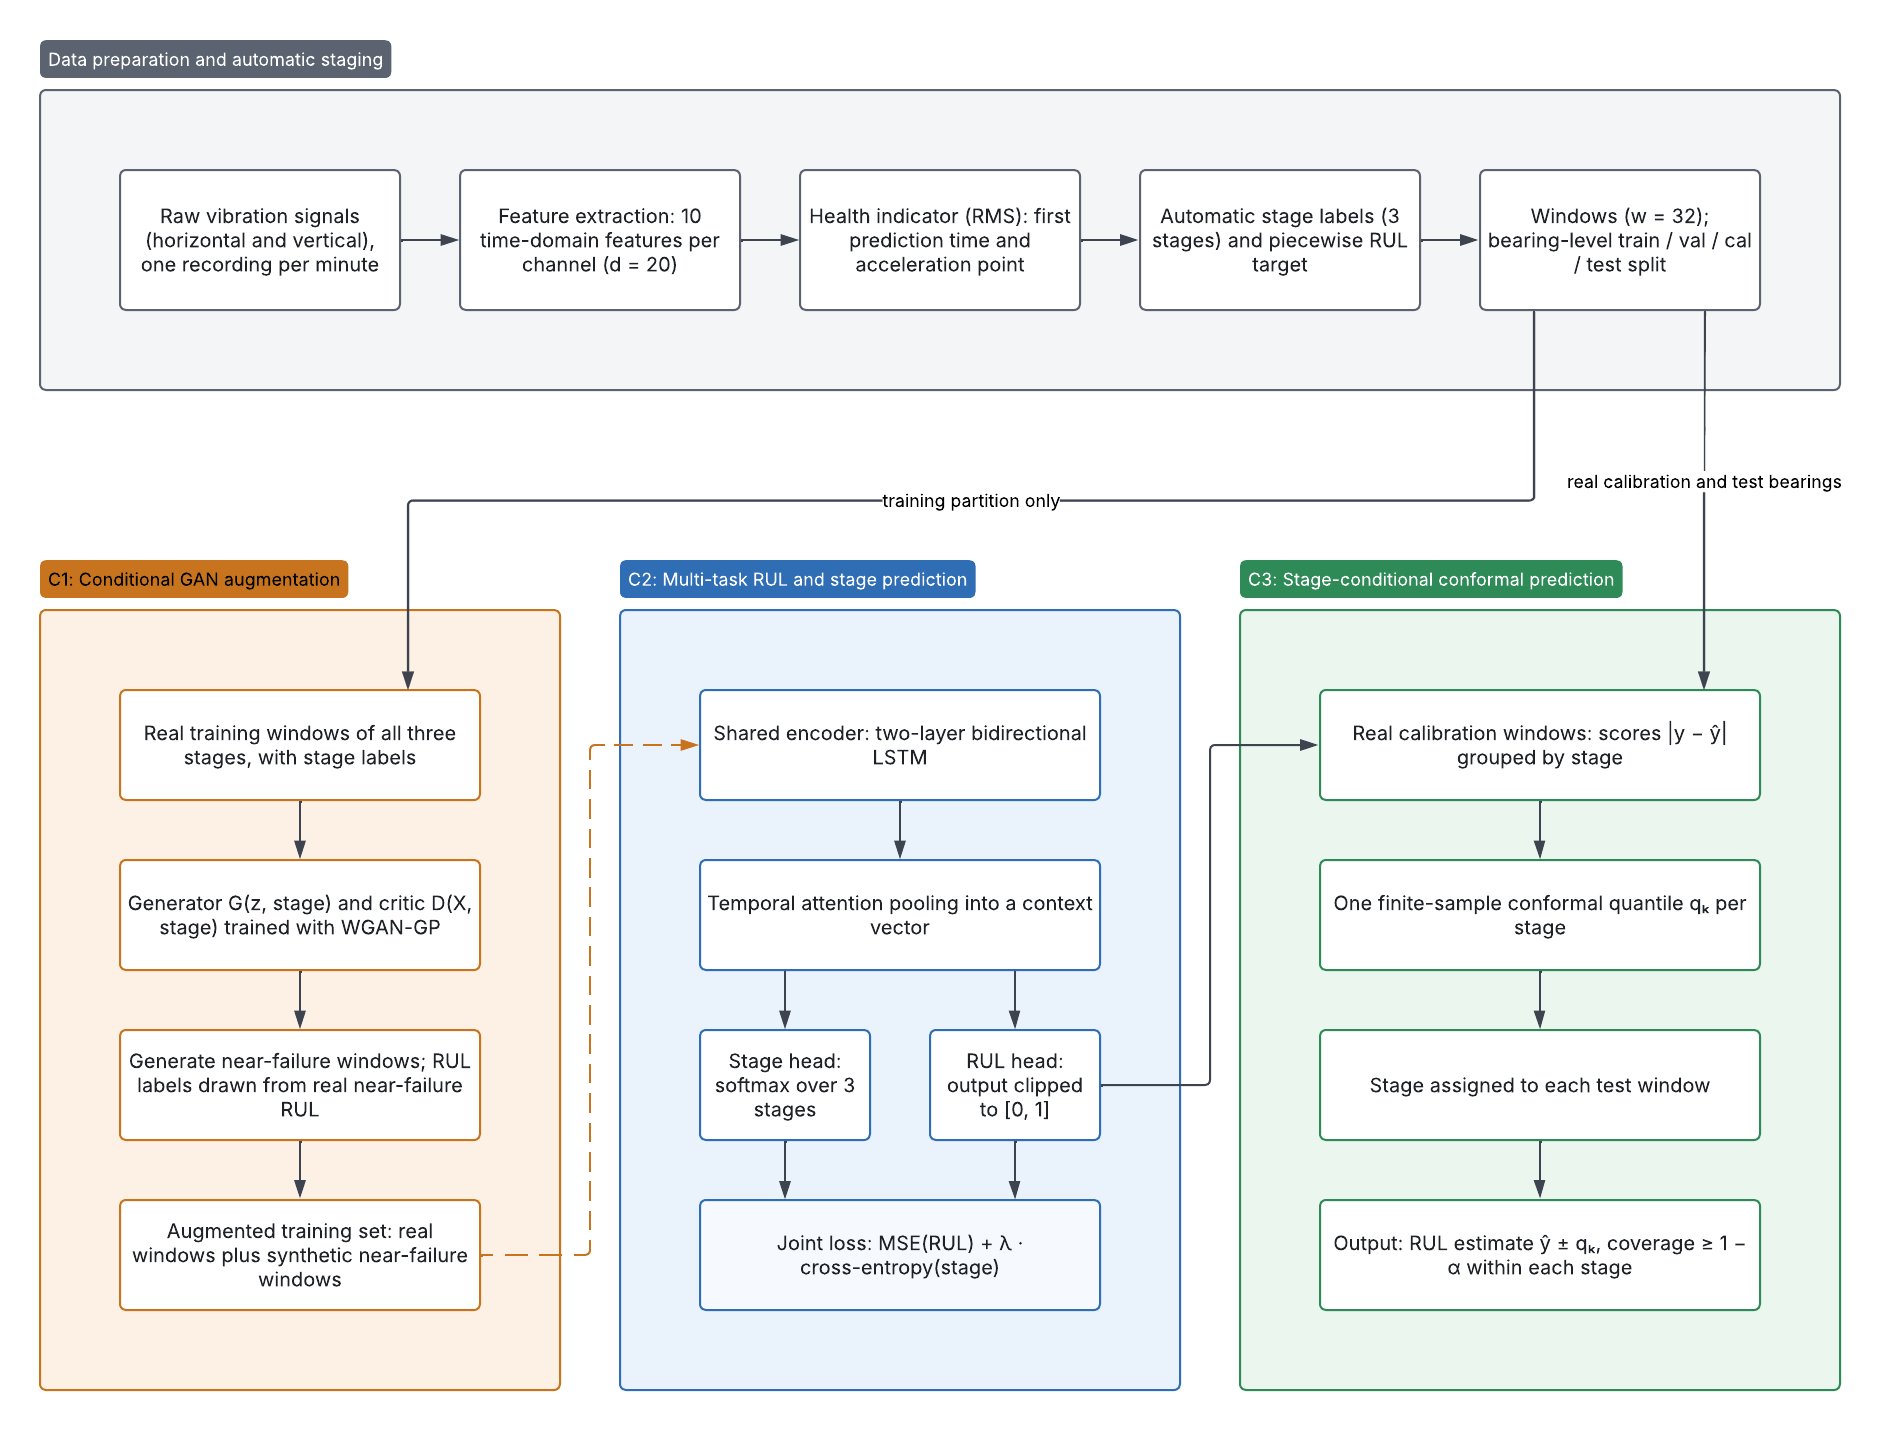
\includegraphics[width=\textwidth]{figures/framework_overview.png}
  \caption{Overview of the proposed framework. Synthetic windows
  produced by the stage-conditioned generator (C1) enter the training
  set only (dashed arrow); calibration and test use real recordings
  exclusively. The RUL head of the multi-task predictor (C2) supplies the
  point estimates whose out-of-sample residuals define the conformal
  intervals, and its stage head supplies the stage on which the interval
  is conditioned (C3).}
  \label{fig:framework}
\end{figure*}

% ------------------------------------------------------------
\subsection{Problem Formulation}
\label{sec:method_notation}

Consider a set of bearings $\mathcal{B}$, each monitored from its
first recording to failure. For bearing $b \in \mathcal{B}$ with
lifetime $T_b$ recordings, a feature vector
$\mathbf{x}^{b}_{t} \in \mathbb{R}^{d}$ is extracted from the
recording at time $t = 1, \dots, T_b$. The model input at time $t$ is
the window of the $w$ most recent feature vectors,
\begin{equation}
  \mathbf{X}^{b}_{t} =
  \left[\mathbf{x}^{b}_{t-w+1}, \dots, \mathbf{x}^{b}_{t}\right]
  \in \mathbb{R}^{w \times d}, \qquad t \geq w,
  \label{eq:window}
\end{equation}
which contains no information posterior to $t$. Each window carries
two labels taken at its final time step: a normalised RUL target
$y^{b}_{t} \in [0,1]$ and a degradation stage
$s^{b}_{t} \in \{1, 2, 3\}$, both defined in
Section~\ref{sec:method_staging}.\\

For a given model, the bearings are split into disjoint training,
validation, calibration and test sets, denoted
$\mathcal{D}_{\mathrm{tr}}$, $\mathcal{D}_{\mathrm{val}}$,
$\mathcal{D}_{\mathrm{cal}}$ and $\mathcal{D}_{\mathrm{te}}$, at the
level of whole bearings. This choice follows from
Eq.~\eqref{eq:window}: consecutive windows of the same bearing share
$w-1$ of their $w$ time steps, so a window-level split would place
near-duplicates on both sides of the training--calibration boundary.
Section~\ref{sec:c3_conformal} describes how these roles rotate among
the non-test bearings.\\

The objective is twofold. The first is a point predictor
$\hat{f}: \mathbb{R}^{w \times d} \to [0,1]$ with small error on
unseen bearings, particularly in the near-failure stage. The second is
an interval predictor $\hat{C}(\mathbf{X})$ that satisfies, for a
user-chosen miscoverage level $\alpha$, the stage-conditional coverage
property
\begin{equation}
  \mathbb{P}\left( y \in \hat{C}(\mathbf{X}) \;\middle|\; s = k \right)
  \geq 1 - \alpha, \qquad k \in \{1, 2, 3\}.
  \label{eq:coverage_goal}
\end{equation}
Coverage within each stage is required, rather than coverage averaged
over all windows, because the stages differ sharply in size and
difficulty. An average dominated by the abundant healthy windows can
satisfy the nominal level while the near-failure stage, the one that
drives maintenance decisions, is under-covered.

% ------------------------------------------------------------
\subsection{Automatic Degradation Staging and RUL Target}
\label{sec:method_staging}

Stage labels and RUL targets are derived from a scalar health
indicator (HI) rather than annotated by hand. The HI $h_t$ is the root
mean square of one vibration channel, computed per recording and
smoothed with a short moving average.\\

The First Prediction Time $t_{\mathrm{F}}$ marks the end of the healthy
regime. A healthy baseline with mean $\mu_b$ and standard deviation
$\sigma_b$ is estimated from the initial fraction $\eta$ of the
bearing's life. The detection threshold is the stricter of a
statistical criterion and a relative floor,
\begin{equation}
  \tau_b = \max\left( \mu_b + 3\sigma_b,\; (1+\rho)\,\mu_b \right),
  \label{eq:fpt_threshold}
\end{equation}
and the FPT is the first instant from which the HI stays above
$\tau_b$ for $m$ consecutive recordings,
\begin{equation}
  t_{\mathrm{F}} = \min \left\{ t \;:\; h_{t+j} > \tau_b,
  \;\; j = 0, \dots, m-1 \right\}.
  \label{eq:fpt}
\end{equation}
The two terms of Eq.~\eqref{eq:fpt_threshold} play distinct roles. The
statistical term rejects departures that are small compared with the
baseline noise. The relative term $\rho$ guards against bearings whose
baseline is so stable that $\sigma_b$ is close to zero, in which case
$\mu_b + 3\sigma_b$ alone would be crossed by ordinary fluctuations.
The persistence length $m$ in Eq.~\eqref{eq:fpt} prevents a single
transient from being taken as a change of regime.\\

Within the degradation phase, an acceleration point $t_{\mathrm{A}}$
separates gradual from severe degradation. Let
$\Delta h_t = h_t - h_{t-1}$ denote the first difference of the HI.
Its mean $\mu_\Delta$ and standard deviation $\sigma_\Delta$ are
estimated over the first half of the interval
$[t_{\mathrm{F}}, T_b]$, and $t_{\mathrm{A}}$ is the first instant in
the second half at which
\begin{equation}
  \Delta h_t > \mu_\Delta + \sigma_\Delta .
  \label{eq:acc_point}
\end{equation}
When no such instant exists, $t_{\mathrm{A}}$ is placed at 70\% of the
degradation interval. The two landmarks define the stage of every
recording,
\begin{equation}
  s_t =
  \begin{cases}
    1 & t < t_{\mathrm{F}} \quad \text{(healthy)},\\
    2 & t_{\mathrm{F}} \leq t < t_{\mathrm{A}}
        \quad \text{(early degradation)},\\
    3 & t \geq t_{\mathrm{A}} \quad \text{(near-failure)}.
  \end{cases}
  \label{eq:stages}
\end{equation}

The RUL target is defined piecewise from the same landmark:
\begin{equation}
  y_t =
  \begin{cases}
    1 & t < t_{\mathrm{F}},\\[2pt]
    \dfrac{T_b - t}{T_b - t_{\mathrm{F}}} & t \geq t_{\mathrm{F}}.
  \end{cases}
  \label{eq:rul_target}
\end{equation}
The target is held at unity during the healthy phase and decreases
linearly to zero at failure. A target that decreases from the first
recording would give different labels to healthy windows whose
signals are nearly identical, a mapping the predictor cannot learn.
Because healthy windows are the most numerous, such a target also
biases the predictor toward overestimating the remaining life, which
is the unsafe direction of error. Normalising by the length of the
degradation phase keeps the target on a common scale across bearings
whose lifetimes may differ by orders of magnitude.

% ------------------------------------------------------------
\subsection{Stage-Conditioned Generative Augmentation (C1)}
\label{sec:c1_gan}

The near-failure stage is the least represented in run-to-failure data
and the most important for maintenance. C1 enlarges it with synthetic
windows produced by a conditional generative adversarial network. The
generator produces complete multivariate windows of dimension
$w \times d$, rather than a scalar degradation curve, so that the
correlations between features and between channels are reproduced.\\

\textit{Architecture.} The generator $G$ receives a noise vector
$\mathbf{z} \sim \mathcal{N}(\mathbf{0}, \mathbf{I})$ concatenated with
a one-hot encoding $\mathbf{e}_c$ of the requested stage $c$. A linear
layer projects this input into a short seed sequence, two
one-dimensional convolutional layers extract local patterns, and a
bidirectional LSTM models the temporal dependencies before a linear
layer outputs the window $\tilde{\mathbf{X}} = G(\mathbf{z},
\mathbf{e}_c)$. The critic $D$ receives a window together with the same
stage encoding, repeated at every time step, and passes it through two
convolutional layers and a bidirectional LSTM. The final hidden state
is layer-normalised and mapped to an unbounded scalar score. Layer
normalisation is used instead of batch normalisation because the
gradient penalty below is defined per sample.\\

Conditioning both networks on the stage is what allows a specific
regime to be requested. An unconditional generator would reproduce the
distribution of its training data, which is dominated by healthy
windows, and leave the scarcity unaddressed. The generator is
therefore trained on windows of all three stages, so that it learns
how the stages differ, and is queried only for $c = 3$ at
augmentation time.\\

\textit{Training objective.} Training follows the Wasserstein
formulation with gradient penalty~\cite{NIPS2017_892c3b1c}, chosen for
its resistance to mode collapse. A collapsed generator would emit
near-identical windows and add no information to the training set.
The critic minimises
\begin{equation}
  \mathcal{L}_{D} =
  \mathbb{E}\big[ D(\tilde{\mathbf{X}}, \mathbf{e}_c) \big]
  - \mathbb{E}\big[ D(\mathbf{X}, \mathbf{e}_c) \big]
  + \lambda_{\mathrm{gp}}\,
  \mathbb{E}\Big[ \big( \lVert \nabla_{\hat{\mathbf{X}}}
  D(\hat{\mathbf{X}}, \mathbf{e}_c) \rVert_2 - 1 \big)^2 \Big],
  \label{eq:critic_loss}
\end{equation}
where $\mathbf{X}$ is a real window of stage $c$, $\tilde{\mathbf{X}}$
a generated window of the same stage, and
$\hat{\mathbf{X}} = \epsilon \mathbf{X} + (1-\epsilon)
\tilde{\mathbf{X}}$ with $\epsilon \sim \mathcal{U}(0,1)$. The last
term enforces the Lipschitz constraint on which the Wasserstein
estimate depends. The generator minimises
\begin{equation}
  \mathcal{L}_{G} =
  - \mathbb{E}\big[ D(G(\mathbf{z}, \mathbf{e}_c), \mathbf{e}_c) \big],
  \label{eq:gen_loss}
\end{equation}
and is updated once for every $n_{\mathrm{c}}$ critic updates. A
separate generator is trained for every predictor, on that predictor's
training windows only, so that no synthetic window derives from a
bearing later used to calibrate it.\\

\textit{Augmentation and labelling.} Let $N_3$ be the number of real
near-failure windows in $\mathcal{D}_{\mathrm{tr}}$. For an
augmentation ratio $r$, the generator produces
$\lfloor r N_3 \rceil$ windows with $c = 3$, and these are added to the
training set with stage label 3. Each synthetic window also needs an
RUL label, which the generator does not provide because it is
conditioned on the stage and not on the RUL. The label is drawn at
random, with replacement, from the empirical distribution of the RUL
values of the real near-failure training windows,
\begin{equation}
  \tilde{y} \sim \mathrm{Unif}\left\{ y_i \;:\; s_i = 3,\;
  i \in \mathcal{D}_{\mathrm{tr}} \right\}.
  \label{eq:syn_label}
\end{equation}
This preserves the marginal distribution of near-failure RUL values in
the augmented set, so the augmentation does not shift the predictor
toward any particular value. The augmented set
$\mathcal{D}_{\mathrm{tr}}^{+} = \mathcal{D}_{\mathrm{tr}} \cup
\mathcal{D}_{\mathrm{syn}}$ replaces $\mathcal{D}_{\mathrm{tr}}$ for
training the predictor. The validation, calibration and test sets are
left unchanged.

% ------------------------------------------------------------
\subsection{Multi-task RUL and Stage Prediction (C2)}
\label{sec:c2_multitask}

The predictor estimates the RUL and the degradation stage jointly from
a shared encoder. The auxiliary stage task asks the encoder to
separate the three regimes, which are the same regimes in which the
RUL behaves differently. The stage labels come from
Eq.~\eqref{eq:stages} and therefore cost no annotation.\\

\textit{Shared encoder.} A two-layer bidirectional LSTM maps the input
window to a sequence of hidden states
$\mathbf{H} = [\mathbf{h}_1, \dots, \mathbf{h}_w]$, where each
$\mathbf{h}_k$ concatenates the forward and backward states. A temporal
attention layer pools this sequence into a context vector,
\begin{equation}
  a_k = \mathbf{v}^{\top} \tanh\left( \mathbf{W}_a \mathbf{h}_k +
  \mathbf{b}_a \right), \qquad
  \beta_k = \frac{\exp(a_k)}{\sum_{j=1}^{w} \exp(a_j)}, \qquad
  \mathbf{c} = \sum_{k=1}^{w} \beta_k \mathbf{h}_k ,
  \label{eq:attention}
\end{equation}
so that the time steps most informative about the current state of
degradation receive the largest weights.\\

\textit{Task heads.} Two heads read the context vector $\mathbf{c}$.
The RUL head is a small feed-forward network whose output is clipped to
the unit interval,
\begin{equation}
  \hat{y} = \min\left( 1, \max\left( 0, \; g_{\mathrm{rul}}(\mathbf{c})
  \right) \right).
  \label{eq:rul_head}
\end{equation}
Clipping is preferred to a sigmoid output because the target of
Eq.~\eqref{eq:rul_target} takes the exact value 1 on every healthy
window, a value a sigmoid only approaches asymptotically. The stage
head is a feed-forward network followed by a softmax over the three
stages, giving the predicted probabilities
$\hat{\mathbf{p}} = \mathrm{softmax}(g_{\mathrm{st}}(\mathbf{c}))$.\\

\textit{Joint objective.} Both heads are trained together on every
window of $\mathcal{D}_{\mathrm{tr}}^{+}$ by minimising
\begin{equation}
  \mathcal{L} = \frac{1}{N} \sum_{i=1}^{N} \left( \hat{y}_i - y_i
  \right)^2
  \;-\; \lambda \, \frac{1}{N} \sum_{i=1}^{N} \log \hat{p}_{i,\,s_i},
  \label{eq:mt_loss}
\end{equation}
where $\lambda \geq 0$ weights the stage loss. Setting $\lambda = 0$
and removing the stage head recovers the single-task predictor used as
the baseline. Healthy windows enter both terms: the piecewise target
makes their RUL learnable, and in the stage term they supply the
examples the encoder needs to recognise the healthy regime. Training
stops when the RUL error on $\mathcal{D}_{\mathrm{val}}$ has not
improved for a fixed number of epochs, and the weights with the lowest
validation error are retained.


% ------------------------------------------------------------
\subsection{Stage-Conditional Cross-Conformal Prediction (C3)}
\label{sec:c3_conformal}

C3 converts the point prediction into an interval with a
distribution-free coverage guarantee. It makes no assumption about the
predictor or the error distribution, and it is applied after training,
so it leaves the predictor unchanged~\cite{lei2018distribution,
angelopoulos2023gentle}.\\

\textit{Split conformal prediction.} In its simplest form, a trained
predictor $\hat{f}$ is applied to a held-out calibration set, and each
calibration window receives the nonconformity score
\begin{equation}
  r_i = \left| y_i - \hat{f}(\mathbf{X}_i) \right|,
  \qquad i \in \mathcal{D}_{\mathrm{cal}} .
  \label{eq:score}
\end{equation}
With the $n$ scores sorted in increasing order,
$r_{(1)} \leq \dots \leq r_{(n)}$, the interval for a new window is
$\hat{f}(\mathbf{X}) \pm \hat{q}$ with
\begin{equation}
  \hat{q} = r_{(k)}, \qquad
  k = \left\lceil (n+1)(1-\alpha) \right\rceil .
  \label{eq:quantile}
\end{equation}
The correction $(n+1)$ yields the finite-sample guarantee
$\mathbb{P}(y \in \hat{C}(\mathbf{X})) \geq 1 - \alpha$ whenever the
calibration and test windows are exchangeable.\\

\textit{Why a single calibration split is insufficient.} Exchangeability
must hold between bearings, not only between windows, because the
windows of one bearing are strongly dependent. A run-to-failure dataset
contains few bearings, and every bearing assigned to calibration is
removed from training. A held-out calibration set therefore represents
the variability between bearings through very few units, and the
intervals inherit whatever is specific to those units. The framework
avoids this by using every non-test bearing for calibration through
cross-conformal prediction.\\

\textit{Cross-conformal calibration (CV+).} The non-test bearings are
divided into $K$ disjoint groups $\mathcal{G}_1, \dots, \mathcal{G}_K$.
For each $j$, a predictor $\hat{f}_{-j}$ is trained without the
bearings of $\mathcal{G}_j$, including its own generator (C1), feature
scaler and early stopping, and is applied to the windows of
$\mathcal{G}_j$. Every non-test window $i$ thus receives an
out-of-sample score
\begin{equation}
  R_i = \left| y_i - \hat{f}_{-j(i)}(\mathbf{X}_i) \right|,
  \label{eq:oof_score}
\end{equation}
where $j(i)$ is the group containing the bearing of window $i$. For a
test window $\mathbf{X}$, each score is combined with the prediction of
the model that produced it, and the CV+
interval~\cite{barber2021jackknife} is
\begin{equation}
  \hat{C}(\mathbf{X}) = \Big[\,
  \hat{q}^{-}_{\alpha}\big\{ \hat{f}_{-j(i)}(\mathbf{X}) - R_i \big\},\;
  \hat{q}^{+}_{\alpha}\big\{ \hat{f}_{-j(i)}(\mathbf{X}) + R_i \big\}
  \,\Big],
  \label{eq:cvplus}
\end{equation}
where, over the $n$ values in braces, $\hat{q}^{+}_{\alpha}$ is the
$\lceil (1-\alpha)(n+1) \rceil$-th smallest value and
$\hat{q}^{-}_{\alpha}$ the $\lfloor \alpha (n+1) \rfloor$-th smallest.
If the $K$ models gave identical predictions, Eq.~\eqref{eq:cvplus}
would reduce to the split interval of Eq.~\eqref{eq:quantile}; it
accounts for their disagreement otherwise. The guarantee is
$1 - 2\alpha$ in the worst case and close to $1 - \alpha$ in
practice~\cite{barber2021jackknife}. The point estimate is the mean of
the $K$ predictions, $\bar{f}(\mathbf{X}) = K^{-1}\sum_j
\hat{f}_{-j}(\mathbf{X})$. Because the RUL lies in $[0,1]$, the
interval is finally intersected with the unit interval, which removes
impossible values without changing coverage.\\

\textit{Conditioning on the predicted stage.} The coverage of
Eq.~\eqref{eq:cvplus} holds on average over all windows, which is
weaker than the requirement of Eq.~\eqref{eq:coverage_goal}. When the
scores of different stages follow different distributions, a single
interval width is too wide for some stages and too narrow for others.
Following the Mondrian construction~\cite{vovk2005algorithmic}, the
calibration windows are partitioned into groups and the quantiles of
Eq.~\eqref{eq:cvplus} are taken within the group of the test window
only. The group must be computable for a bearing in service. The
landmarks of Section~\ref{sec:method_staging} are located from the
complete trajectory, so the true stage is not available before failure.
The group is therefore the stage predicted from the window,
$\hat{s} = \arg\max_k \hat{p}_k$. Each calibration window takes the
stage predicted by the stage head of the model that did not see it,
and a test window takes the stage that maximises the average of the
$K$ stage heads' probabilities. Because $\hat{s}$ depends on the input
only, the guarantee holds within each predicted stage; coverage within
the true stages is measured empirically in Section~\ref{sec:results}.\\

In the multi-task configurations this links C2 and C3 directly: the
stage head that shapes the shared representation during training also
supplies the stage on which the interval is conditioned, so a single
network provides the RUL estimate, the stage and the interval. In the
single-task configurations, which have no stage head, the stage is
provided by a separate network with the same encoder and stage head,
trained on the same real training windows.\\

Three design choices protect the exchangeability on which these
guarantees rest. Partitioning is done at the bearing level, so that no
calibration window has a near-duplicate in the training data of the
model that scores it. Synthetic windows are confined to training, and
each generator is trained only on the bearings of its own predictor,
so that calibration measures the error against real, unseen data.
Finally, every non-test bearing contributes to calibration, so that
the calibration population reflects the variability between bearings
as fully as the dataset allows.

% ------------------------------------------------------------
\subsection{Training and Evaluation Procedure}
\label{sec:method_procedure}

Algorithm~\ref{alg:framework} summarises the procedure for one set of
test bearings. The four configurations compared in
Section~\ref{sec:results} are obtained by switching C1 and C2 on or
off: the baseline uses neither ($r = 0$, $\lambda = 0$), the augmented
configuration uses C1 only, the multi-task configuration uses C2 only,
and the full framework uses both. C3 is applied identically to all
four, so that differences in the intervals can be attributed to the
predictor.

\begin{algorithm}[!htbp]
\caption{Proposed framework for one set of test bearings.}
\label{alg:framework}
\begin{algorithmic}[1]
\Require Test bearings $\mathcal{D}_{\mathrm{te}}$; non-test bearings
         in groups $\mathcal{G}_1, \dots, \mathcal{G}_K$; ratio $r$;
         weight $\lambda$; level $\alpha$
\State Compute $t_{\mathrm{F}}$, $t_{\mathrm{A}}$, $s_t$ and $y_t$ for
       every bearing \Comment{Eqs.~\eqref{eq:fpt}--\eqref{eq:rul_target}}
\For{$j = 1, \dots, K$}
  \State $\mathcal{D}_{\mathrm{tr}}, \mathcal{D}_{\mathrm{val}} \gets$
         non-test bearings outside $\mathcal{G}_j$
  \State Fit the feature scaler on $\mathcal{D}_{\mathrm{tr}}$
  \If{$r > 0$} \Comment{C1}
    \State Train $(G, D)$ on $\mathcal{D}_{\mathrm{tr}}$; generate
           $\lfloor r N_3 \rceil$ windows with $c=3$, labelled by
           Eq.~\eqref{eq:syn_label}
  \EndIf
  \State Train $\hat{f}_{-j}$ on $\mathcal{D}_{\mathrm{tr}}^{+}$ with
         Eq.~\eqref{eq:mt_loss}; early-stop on $\mathcal{D}_{\mathrm{val}}$
         \Comment{C2}
  \State Score $\mathcal{G}_j$: $R_i$ by Eq.~\eqref{eq:oof_score} and
         $\hat{s}_i$ from the stage head
  \State Predict $\mathcal{D}_{\mathrm{te}}$: RUL and stage probabilities
\EndFor
\For{each $\mathbf{X} \in \mathcal{D}_{\mathrm{te}}$} \Comment{C3}
  \State $\hat{s} \gets$ stage of the averaged probabilities;
         $\bar{f}(\mathbf{X}) \gets$ mean of the $K$ predictions
  \State $\hat{C}(\mathbf{X}) \gets$ Eq.~\eqref{eq:cvplus} over the
         calibration windows with $\hat{s}_i = \hat{s}$, clipped to $[0,1]$
\EndFor
\end{algorithmic}
\end{algorithm}

% ============================================================
%  Section 4 — Experimental Setup
%  Dataset-specific choices and the evaluation protocol. The
%  framework itself is defined in Section 3; measured outcomes are
%  in Section 5.
% ============================================================

\section{Experimental Setup}
\label{sec:experimental_setup}

% ------------------------------------------------------------
\subsection{Dataset Description}
\label{sec:dataset}

The framework is evaluated on the XJTU-SY rolling element bearing
dataset~\cite{8576668, lei2019xjtusy}, a widely used benchmark that
provides complete run-to-failure vibration data from accelerated life
tests. The dataset comprises 15~bearings in three groups of five, each
tested under a distinct operating condition
(Table~\ref{tab:xjtu_conditions}). Two accelerometers record the
horizontal and vertical vibration simultaneously. Each recording lasts
1.28~s (32,768~samples at 25.6~kHz) and is taken once per minute until
failure.

\begin{table}[htbp]
\centering
\caption{XJTU-SY operating conditions and bearing characteristics.}
\label{tab:xjtu_conditions}
\footnotesize
\renewcommand{\arraystretch}{1.2}
\begin{tabular}{cccccc}
\toprule
\textbf{Cond.} & \textbf{Speed} & \textbf{Load} &
\textbf{Bearings} & \textbf{Lifetime range} &
\textbf{Failure modes} \\
& (Hz) & (kN) & & (min) & \\
\midrule
1 & 35.0  & 12.0 & 1-1 to 1-5 & 52--161 &
  OR (3), Cage (1), OR+Ball (1) \\
2 & 37.5  & 11.0 & 2-1 to 2-5 & 42--533 &
  OR (3), IR (1), Cage (1) \\
3 & 40.0  & 10.0 & 3-1 to 3-5 & 114--2538 &
  OR (2), IR (2), IR+Ball (1) \\
\bottomrule
\end{tabular}

\vspace{2pt}
\raggedright\scriptsize OR: outer race. IR: inner race.
\end{table}

Bearing lifetimes vary widely across and within operating conditions
(Fig.~\ref{fig:lifetime_distribution}). Condition~1, with the heaviest
radial load, produces the shortest lifetimes (52--161~min), while
Condition~3 ranges from 114 to over 2,500~min. Within Condition~2,
Bearing~2-4 failed after 42~min and Bearing~2-3 after 533~min under
identical settings. Failure modes also differ between bearings of the
same condition, so the operating parameters influence the failure mode
without determining it.\\

\begin{figure}[htbp]
  \centering
  \includegraphics[width=\columnwidth]{figures/01_lifetime_distribution.png}
  \caption{Bearing lifetimes across the three operating conditions
  of the XJTU-SY dataset.}
  \label{fig:lifetime_distribution}
\end{figure}

Fig.~\ref{fig:all_bearings_rms} shows the RMS of the horizontal
channel over the life of all 15~bearings. The RMS stays near a low
baseline during healthy operation, rises as degradation starts, and
climbs sharply before failure. The dynamics nonetheless differ between
bearings: smooth monotone growth (Bearing~3-1), abrupt failure with
little warning (Bearing~1-4, cage fault), oscillation with partial
recoveries (Bearing~2-5), or several distinct rates of change
(Bearing~1-2). A predictor must learn from all of these patterns, and
an interval must remain valid across them.

\begin{figure}[htbp]
  \centering
  \includegraphics[width=\columnwidth]{figures/01_all_15_bearings_rms_overview.png}
  \caption{RMS vibration amplitude (horizontal channel) over the
  operational life of all 15~XJTU-SY bearings, organised by operating
  condition, with bearing ID, failure mode and lifetime.}
  \label{fig:all_bearings_rms}
\end{figure}

% ------------------------------------------------------------
\subsection{Health Indicator, Stage Labels and Features}
\label{sec:hi_staging}

The health indicator of Section~\ref{sec:method_staging} is the RMS of
the horizontal channel, which responds most strongly to the radial
load applied in these tests~\cite{lu_joint_2022}, smoothed with a
short moving average. The healthy baseline is estimated over the first
$\eta = 20\%$ of each bearing's life, the relative floor is
$\rho = 0.20$, and the persistence length is $m = 5$ recordings.\\

The relative floor is necessary on this dataset. Long-lived bearings
have an exceptionally stable baseline: for Bearing~3-1 the healthy RMS
varies by only a few percent, so $\mu + 3\sigma$ lies barely above the
healthy level and is crossed by ordinary fluctuations. Without the
floor, the FPT of Bearing~3-1 is detected at minute~23 of 2,537,
labelling more than 99\% of its life as degrading, and that of
Bearing~3-2 at minute~169 of 2,495. These two bearings hold over half
of all recordings, so the error would propagate into every partition.
Across the 15~bearings, healthy fluctuations remain within about 10\%
of the baseline, whereas degradation raises the RMS by close to an
order of magnitude, so a 20\% floor separates the two regimes with a
wide margin.\\

Fig.~\ref{fig:hi_all_bearings} overlays the resulting stages on the
health indicator. In every bearing the onset of Stage~2 coincides with
the visible departure from the baseline and Stage~3 with the terminal
rise. Two groups of bearings appear. Some degrade abruptly, with a flat
indicator for most of their life and a near-vertical rise that
compresses both degradation stages into a short final window
(Bearings~2-1, 3-1, 3-3 and~3-4). Others degrade progressively, often
with oscillations (Bearings~1-2, 2-3, 2-5 and~3-2). Abrupt failures
occur in short- and long-lived bearings alike, which is why the
threshold is expressed in relative terms.

\begin{figure}[htbp]
  \centering
  \includegraphics[width=\textwidth]{figures/02_all_bearings_stages.png}
  \caption{Health indicator (horizontal RMS) of all 15~bearings with
  the automatically detected stages. Green: Stage~1 (healthy). Orange:
  Stage~2 (early degradation). Red: Stage~3 (near-failure). Dashed
  lines: FPT and acceleration point.}
  \label{fig:hi_all_bearings}
\end{figure}

Over all 9,216~recordings, Stage~1 accounts for 70.7\%, Stage~2 for
15.9\% and Stage~3 for only 13.4\% (Fig.~\ref{fig:stage_distribution}).
The imbalance is stronger still within bearings: several bearings
contribute only a handful of near-failure recordings, and Bearing~3-2
alone holds about half of all near-failure windows. This is the
scarcity that C1 targets, and the concentration that makes calibration
on few bearings fragile.

\begin{figure}[htbp]
  \centering
  \includegraphics[width=\columnwidth]{figures/02_stage_distribution_per_bearing_pct.png}
  \caption{Degradation stage distribution. Left: composition of each
  bearing's life. Right: global composition over all 9,216~recordings.}
  \label{fig:stage_distribution}
\end{figure}

The predictors use a multivariate representation. Ten time-domain
features are extracted per channel and recording: amplitude
descriptors (RMS, peak, peak-to-peak, standard deviation),
distribution-shape descriptors (kurtosis, skewness) and dimensionless
impulse descriptors (crest, shape, impulse and clearance factors).
The two channels give $d = 20$ features per recording.
Fig.~\ref{fig:feature_matrix} shows that these features are stable
during the healthy phase and change sharply from the FPT onward, with
amplitude and distribution-shape descriptors moving in opposite
directions. The feature families therefore carry complementary
information, which motivates generating and predicting from the full
multivariate window rather than a scalar indicator.

\begin{figure}[htbp]
  \centering
  \includegraphics[width=\columnwidth]{figures/02_feature_matrix_heatmap.png}
  \caption{Temporal evolution of the 20 time-domain features (z-scored
  per feature) for Bearing~2-1. Dashed lines: FPT and acceleration
  point.}
  \label{fig:feature_matrix}
\end{figure}

% ------------------------------------------------------------
\subsection{Windowing, Normalisation and Partitioning}
\label{sec:windowing}

Windows of $w = 32$ recordings are taken with a stride of one, giving
inputs of dimension $32 \times 20$. The unit stride is kept despite the
overlap between adjacent windows because the shortest bearings would
otherwise contribute almost nothing: Bearing~2-4 yields only
11~windows even at unit stride.\\

The amplitude, impulse and kurtosis features are strictly positive and
grow by about a factor of twenty near failure. They are log-transformed
before standardisation, which would otherwise be dominated by the
abundant healthy windows and place near-failure values tens of
standard deviations from the mean. Standardisation statistics are
estimated on the training windows of each model only, and the
standardised values are clipped to $\pm 5$ standard deviations to bound
the low-variance shape features.\\

\textit{Outer folds.} Five folds are formed following the protocol of
Lu et al.~\cite{lu_joint_2022}: fold~$k$ tests on Bearings~1-$k$, 2-$k$
and~3-$k$, so that every fold spans the three operating conditions and
every bearing is tested exactly once.\\

\textit{Inner groups for cross-conformal calibration.} The 12 non-test
bearings of each fold contain four bearings per operating condition.
They are divided into $K = 4$ groups of three, group~$j$ holding the
$j$-th remaining bearing of each condition, so that every inner model
is trained on all three conditions, as the test set is. Each inner
model therefore trains on 9~bearings and scores its 3~held-out
bearings. Of the 9, one is used for early stopping: the smallest
bearing that yields at least 300~windows, so that the validation error
is stable enough to detect a genuine plateau, while as few windows as
possible are withheld from training. The remaining 8~bearings form the
training set. Over the 12 non-test bearings, the four inner models
provide out-of-sample residuals for every window.\\

Because three bearings account for most of the recordings, the folds
remain unbalanced after partitioning: test sets range from 412 to
3,059~windows. Per-fold metrics are therefore estimated with unequal
precision, which is why results are also examined per bearing
(Section~\ref{sec:res_per_bearing}).

% ------------------------------------------------------------
\subsection{Implementation Details}
\label{sec:implementation}

Table~\ref{tab:hyperparams} lists the hyperparameters. The augmentation
ratio $r = 0.75$ and the stage-loss weight $\lambda = 1.0$ were
selected on preliminary runs over $r \in \{0.25, 0.5, 0.75, 1.0\}$ and
$\lambda \in \{0.3, 0.5, 1.0\}$. A generator is trained for each of the
20 inner models (5 folds $\times$ 4 groups); it does not depend on the
seed. In the single-task configurations, the stage used by C3 comes
from a stage network identical in architecture and training to the
multi-task predictor without augmentation.

\begin{table}[htbp]
\centering
\caption{Hyperparameters of the framework components.}
\label{tab:hyperparams}
\footnotesize
\renewcommand{\arraystretch}{1.15}
\begin{tabular}{lll}
\toprule
\textbf{Component} & \textbf{Setting} & \textbf{Value} \\
\midrule
\multirow{8}{*}{C1 (generator, critic)}
 & Noise dimension & 64 \\
 & Conv.\ channels / kernel & 128 / 5 \\
 & BiLSTM units per direction & 128 \\
 & Optimiser, learning rate & Adam, $10^{-4}$ \\
 & Adam $(\beta_1, \beta_2)$ & $(0.5, 0.9)$ \\
 & Batch size / epochs & 64 / 300 \\
 & Critic steps $n_{\mathrm{c}}$ & 3 \\
 & Penalty weight $\lambda_{\mathrm{gp}}$ & 10 \\
\midrule
\multirow{8}{*}{C2 (predictor)}
 & BiLSTM layers / units & 2 / 48 \\
 & Head hidden units & 48 \\
 & Dropout & 0.4 \\
 & Optimiser, learning rate & Adam, $5 \times 10^{-4}$ \\
 & Weight decay & $5 \times 10^{-4}$ \\
 & Batch / max.\ epochs / patience & 64 / 100 / 25 \\
 & Gradient clipping (norm) & 5.0 \\
 & Stage-loss weight $\lambda$ & 1.0 \\
\midrule
Augmentation & Ratio $r$ & 0.75 \\
\multirow{2}{*}{C3 (conformal)} & Inner groups $K$ & 4 \\
 & Miscoverage $\alpha$ & 0.10\textsuperscript{a} \\
\bottomrule
\end{tabular}

\vspace{2pt}
\raggedright\scriptsize \textsuperscript{a}Headline level; 0.05, 0.15
and 0.20 are also evaluated.
\end{table}

All models were implemented in PyTorch and trained on a single NVIDIA
T4 GPU. Recurrent training on the GPU is not bit-wise reproducible, and
the RUL error of a given configuration varies by about
$\pm 0.015$--$0.02$ from run to run. Every configuration is therefore
trained under five seeds; with 5~folds and 4~inner models, each
configuration comprises 100 trained predictors. Results are the mean
and standard deviation over seeds of the fold-averaged metrics, and a
difference smaller than the seed-to-seed variability is not interpreted
as an effect.

% ------------------------------------------------------------
\subsection{Evaluation Metrics}
\label{sec:metrics}

Point accuracy is the root mean square error on the normalised RUL
scale, computed per test bearing and then averaged, so that the
long-lived bearings, which supply most windows, do not dominate:
\begin{equation}
  \mathrm{RMSE} = \frac{1}{|\mathcal{B}_{\mathrm{te}}|}
  \sum_{b \in \mathcal{B}_{\mathrm{te}}}
  \sqrt{ \frac{1}{|\mathcal{W}_b|} \sum_{t \in \mathcal{W}_b}
  \left( \hat{y}^{b}_{t} - y^{b}_{t} \right)^2 } ,
  \label{eq:rmse}
\end{equation}
where $\mathcal{W}_b$ is the set of evaluated windows of bearing $b$.
Interval quality is measured by the prediction interval coverage
probability and the mean prediction interval width,
\begin{equation}
  \mathrm{PICP} = \frac{1}{n} \sum_{i=1}^{n}
  \mathbb{1}\left\{ y_i \in \hat{C}(\mathbf{X}_i) \right\},
  \qquad
  \mathrm{MPIW} = \frac{1}{n} \sum_{i=1}^{n}
  \left| \hat{C}(\mathbf{X}_i) \right| ,
  \label{eq:picp_mpiw}
\end{equation}
computed over the test windows of each fold, with intervals clipped to
$[0,1]$. PICP should lie at or slightly above $1-\alpha$, and a smaller
MPIW is better only when PICP is maintained, so the two are always
reported together. All metrics are reported for the healthy, early and
near-failure stages, for the post-FPT windows and for all windows.
Stage subsets are always defined by the true stage, so that the
configurations are compared on the same windows.\\

Three versions of C3 are compared, all built on the same CV+
residuals: a single quantile for all windows; quantiles per
\emph{predicted} stage, which is the deployable framework; and
quantiles per \emph{true} stage, which uses information available only
after failure and serves as a reference for what perfect stage
recognition would achieve. The stage prediction itself is assessed by
its accuracy and by the recall and precision of the near-failure
stage.

% ============================================================
%  Section 5 — Results
%  Measured outcomes only; the methods are defined in Sections 3-4.
%  All figures: XJTU-SY, 5 outer folds, 5 seeds, alpha = 0.10 unless
%  stated; mean +/- std over seeds of the fold-averaged metrics.
%  Source: repo results/09_cvplus (paper_tables.json,
%  per_bearing_report.md) and results/c3_offline.
% ============================================================

\section{Results}
\label{sec:results}

% ------------------------------------------------------------
\subsection{Synthetic Near-Failure Windows}
\label{sec:res_gan}

The synthetic near-failure windows were assessed on four criteria
before entering training: separability from real windows, diversity,
location in a two-dimensional embedding, and per-feature marginal
distributions. Table~\ref{tab:gan_quality} reports the first two for
the generators of the five outer folds, trained on the same
configuration as the inner generators.

\begin{table}[htbp]
\centering
\caption{Quality of the synthetic near-failure windows per fold.
Separability: accuracy of a classifier separating real from synthetic
windows (50\% = indistinguishable). Diversity ratio: mean pairwise
distance among synthetic windows divided by that among real windows
(1 = matched diversity).}
\label{tab:gan_quality}
\footnotesize
\renewcommand{\arraystretch}{1.2}
\begin{tabular}{cccccc}
\toprule
& \multicolumn{5}{c}{\textbf{Fold}} \\
\cmidrule(lr){2-6}
\textbf{Metric} & 1 & 2 & 3 & 4 & 5 \\
\midrule
Separability (\%) & 67.7 & 59.1 & 61.5 & 70.2 & 64.7 \\
Diversity ratio   & 0.82 & 0.78 & 0.81 & 0.78 & 0.87 \\
\bottomrule
\end{tabular}
\end{table}

Separability stays between 59\% and 70\%, approaching chance in the
folds richest in near-failure data, and the diversity ratio between
0.78 and 0.87, so the generator reproduces the spread of the real data
without mode collapse. In the embedding of Fig.~\ref{fig:tsne}, the
synthetic windows occupy the same regions as the real ones in every
fold, including the small isolated sub-populations, and form no
separate cluster. The per-feature distributions of
Fig.~\ref{fig:feature_dist} coincide for all twenty features,
including the bimodal shape of the amplitude features near failure.

\begin{figure}[htbp]
  \centering
  \includegraphics[width=\textwidth]{figures/04_tsne_real_vs_synthetic.png}
  \caption{t-SNE embedding of real (blue) and synthetic (red)
  near-failure windows for each fold.}
  \label{fig:tsne}
\end{figure}

\begin{figure}[htbp]
  \centering
  \includegraphics[width=\columnwidth]{figures/04_feature_distributions.png}
  \caption{Per-feature distributions of real and synthetic near-failure
  windows for a representative fold.}
  \label{fig:feature_dist}
\end{figure}

Two labelling schemes for the synthetic windows were compared in an
exploratory sweep (Table~\ref{tab:aug_sweep}): the label of the nearest
real near-failure window in feature space, and the sampling scheme of
Eq.~\eqref{eq:syn_label}. The nearest-neighbour scheme shifted the
synthetic labels upward (mean 0.27 against 0.24 for real windows),
pushing the predictor toward overestimating the remaining life. The
sampling scheme matched the real mean within 0.01 in every fold and
gave a lower error at every ratio, with its minimum at $r = 0.75$. A
control in which real near-failure windows were duplicated instead of
synthesised gave no improvement (near-failure RMSE 0.247 at ratio 0.5
and 0.250 at ratio 1.0), which indicates that the predictor was not
limited by the number of near-failure windows as such.

\begin{table}[htbp]
\centering
\caption{Exploratory sweep (single run per setting) of near-failure
RMSE by labelling scheme and augmentation ratio.}
\label{tab:aug_sweep}
\footnotesize
\renewcommand{\arraystretch}{1.2}
\begin{tabular}{lcccc}
\toprule
\textbf{Scheme} & \textbf{0.25} & \textbf{0.50} & \textbf{0.75} & \textbf{1.00} \\
\midrule
Sampling          & 0.272 & 0.247 & \textbf{0.231} & 0.232 \\
Nearest-neighbour & 0.266 & 0.265 & 0.239 & 0.243 \\
\bottomrule
\end{tabular}
\end{table}

% ------------------------------------------------------------
\subsection{Point Accuracy and Stage Recognition}
\label{sec:res_accuracy}

Table~\ref{tab:rmse} reports the RMSE of the four configurations by
stage. Multi-task learning is the component that improves accuracy.
It lowers the near-failure RMSE from 0.225 to 0.216, and to 0.206 when
combined with augmentation, the lowest and least variable value. The
effect is larger over the whole life: the overall RMSE falls from 0.385
to 0.297 with C2 and to 0.291 with both components. Most of this gain
comes from the healthy windows, whose error is the largest and most
variable in the baseline (0.392 $\pm$ 0.290) and drops to about 0.26
with C2. Augmentation alone leaves the near-failure RMSE unchanged
(0.226) and lowers the overall RMSE from 0.385 to 0.347, a difference
within the seed-to-seed variability of that metric.

\begin{table}[htbp]
\centering
\caption{RMSE (normalised RUL, per bearing) by stage, mean $\pm$
standard deviation over five seeds. Point estimate: mean of the four
inner models.}
\label{tab:rmse}
\footnotesize
\renewcommand{\arraystretch}{1.2}
\setlength{\tabcolsep}{4pt}
\begin{tabular}{lccccc}
\toprule
\textbf{Config.} & \textbf{Healthy} & \textbf{Early} &
\textbf{Near-failure} & \textbf{Post-FPT} & \textbf{All} \\
\midrule
Baseline & $0.392 \pm 0.290$ & $0.360 \pm 0.120$ & $0.225 \pm 0.041$ & $0.339 \pm 0.068$ & $0.385 \pm 0.161$ \\
+GAN     & $0.337 \pm 0.226$ & $0.329 \pm 0.084$ & $0.226 \pm 0.038$ & $0.313 \pm 0.042$ & $0.347 \pm 0.121$ \\
+MT      & $0.261 \pm 0.173$ & $0.280 \pm 0.068$ & $0.216 \pm 0.035$ & $0.284 \pm 0.045$ & $0.297 \pm 0.101$ \\
+GAN+MT  & $0.266 \pm 0.166$ & $0.280 \pm 0.075$ & $\mathbf{0.206 \pm 0.026}$ & $\mathbf{0.275 \pm 0.041}$ & $\mathbf{0.291 \pm 0.098}$ \\
\bottomrule
\end{tabular}
\end{table}

The stage on which C3 is conditioned is recognised with an accuracy of
$0.722 \pm 0.021$ by the stage network of the configurations without
augmentation, and $0.706 \pm 0.018$ by the stage head of the full
framework. Near-failure windows are found reliably, with a recall of
$0.887 \pm 0.018$ and $0.896 \pm 0.034$ respectively, but the
precision is lower ($0.730 \pm 0.025$ and $0.674 \pm 0.042$): the
main error is to assign early-degradation windows to the near-failure
stage.

% ------------------------------------------------------------
\subsection{Calibration on Two Bearings versus Cross-Conformal Calibration}
\label{sec:res_calibration}

To measure the effect of the calibration scheme, the configurations
were also calibrated by split conformal prediction, with one predictor
per fold trained on 9~bearings and two held-out calibration bearings
chosen to contain at least 100 near-failure windows and a stage
composition close to the test set. Table~\ref{tab:calibration}
compares this protocol with CV+ for the baseline and the full
framework.

\begin{table*}[!htbp]
\centering
\caption{Coverage and width at a 90\% target under split conformal
calibration on two bearings and under cross-conformal (CV+)
calibration on twelve bearings. PICP $\pm$ std over seeds / MPIW.}
\label{tab:calibration}
\scriptsize
\renewcommand{\arraystretch}{1.2}
\setlength{\tabcolsep}{4pt}
\begin{tabular}{llcccc}
\toprule
& & \multicolumn{2}{c}{\textbf{Baseline}} & \multicolumn{2}{c}{\textbf{+GAN+MT}} \\
\cmidrule(lr){3-4}\cmidrule(lr){5-6}
\textbf{Calibration} & \textbf{Grouping} & \textbf{All} & \textbf{Near-failure} & \textbf{All} & \textbf{Near-failure} \\
\midrule
\multirow{3}{*}{Split, 2 bearings}
 & Single $q$        & $0.793 \pm 0.069$ / 0.68 & $0.871 \pm 0.105$ / 0.69 & $0.830 \pm 0.050$ / 0.59 & $0.839 \pm 0.080$ / 0.63 \\
 & Predicted stage   & $0.740 \pm 0.022$ / 0.63 & $0.887 \pm 0.046$ / 0.65 & $0.817 \pm 0.047$ / 0.54 & $0.884 \pm 0.046$ / 0.67 \\
 & True stage        & $0.786 \pm 0.052$ / 0.55 & $0.860 \pm 0.027$ / 0.47 & $0.811 \pm 0.034$ / 0.46 & $0.864 \pm 0.025$ / 0.49 \\
\midrule
\multirow{3}{*}{CV+, 12 bearings}
 & Single $q$        & $0.898 \pm 0.087$ / 0.84 & $0.971 \pm 0.029$ / 0.88 & $0.856 \pm 0.043$ / 0.75 & $0.959 \pm 0.024$ / 0.79 \\
 & Predicted stage   & $\mathbf{0.909 \pm 0.040}$ / 0.67 & $0.968 \pm 0.028$ / 0.83 & $\mathbf{0.917 \pm 0.039}$ / 0.60 & $0.954 \pm 0.023$ / 0.84 \\
 & True stage        & $0.898 \pm 0.065$ / 0.76 & $0.905 \pm 0.027$ / 0.54 & $0.880 \pm 0.038$ / 0.69 & $0.910 \pm 0.014$ / 0.55 \\
\bottomrule
\end{tabular}
\end{table*}

Calibrated on two bearings, every version under-covers: overall
coverage lies between 0.74 and 0.83, and even the true stage gives only
0.79--0.81 overall and 0.86 near failure. The intervals are narrow
because they are calibrated on two bearings that do not represent the
test bearings. Under CV+, coverage returns to the nominal level: the
predicted-stage version reaches 0.909 and 0.917 overall, and the
true-stage version 0.905 and 0.910 near failure. The intervals are
wider than under split calibration, which is the expected price of
calibrating against the full variability of the non-test bearings.
All remaining results use CV+.

% ------------------------------------------------------------
\subsection{Interval Quality and Stage Conditioning}
\label{sec:res_intervals}

Table~\ref{tab:intervals} compares the three versions of C3 for the
four configurations.

\begin{table*}[!htbp]
\centering
\caption{CV+ coverage and width at a 90\% target by grouping and
configuration. PICP $\pm$ std over seeds / MPIW (clipped). Stage
subsets are defined by the true stage. The predicted stage comes from
the model's own stage head (+MT, +GAN+MT) or from the separate stage
network (baseline, +GAN).}
\label{tab:intervals}
\scriptsize
\renewcommand{\arraystretch}{1.2}
\setlength{\tabcolsep}{2.5pt}
\begin{tabular}{llccccc}
\toprule
\textbf{Config.} & \textbf{Grouping} & \textbf{Healthy} & \textbf{Early} &
\textbf{Near-failure} & \textbf{Post-FPT} & \textbf{All} \\
\midrule
\multirow{3}{*}{Baseline}
 & Single $q$      & $0.825 \pm 0.153$ / 0.83 & $0.902 \pm 0.080$ / 0.87 & $0.971 \pm 0.029$ / 0.88 & $0.932 \pm 0.057$ / 0.87 & $0.898 \pm 0.087$ / 0.84 \\
 & Predicted stage & $0.900 \pm 0.037$ / 0.62 & $0.819 \pm 0.100$ / 0.77 & $0.968 \pm 0.028$ / 0.83 & $0.885 \pm 0.067$ / 0.80 & $0.909 \pm 0.040$ / 0.67 \\
 & True stage      & $0.827 \pm 0.153$ / 0.80 & $0.944 \pm 0.013$ / 0.88 & $0.905 \pm 0.027$ / 0.54 & $0.925 \pm 0.013$ / 0.73 & $0.898 \pm 0.065$ / 0.76 \\
\midrule
\multirow{3}{*}{+GAN}
 & Single $q$      & $0.846 \pm 0.086$ / 0.86 & $0.901 \pm 0.079$ / 0.88 & $0.972 \pm 0.028$ / 0.90 & $0.932 \pm 0.055$ / 0.89 & $0.905 \pm 0.064$ / 0.86 \\
 & Predicted stage & $0.799 \pm 0.062$ / 0.60 & $0.851 \pm 0.088$ / 0.80 & $0.969 \pm 0.028$ / 0.82 & $0.903 \pm 0.057$ / 0.81 & $0.872 \pm 0.030$ / 0.66 \\
 & True stage      & $0.853 \pm 0.086$ / 0.84 & $0.939 \pm 0.020$ / 0.89 & $0.908 \pm 0.022$ / 0.54 & $0.923 \pm 0.021$ / 0.74 & $0.904 \pm 0.045$ / 0.79 \\
\midrule
\multirow{3}{*}{+MT}
 & Single $q$      & $0.807 \pm 0.100$ / 0.73 & $0.833 \pm 0.100$ / 0.79 & $0.955 \pm 0.044$ / 0.79 & $0.886 \pm 0.075$ / 0.79 & $0.860 \pm 0.076$ / 0.74 \\
 & Predicted stage & $0.931 \pm 0.013$ / 0.53 & $0.759 \pm 0.089$ / 0.67 & $0.960 \pm 0.025$ / 0.80 & $0.847 \pm 0.057$ / 0.73 & $0.909 \pm 0.026$ / 0.60 \\
 & True stage      & $0.807 \pm 0.100$ / 0.69 & $0.911 \pm 0.040$ / 0.86 & $0.893 \pm 0.007$ / 0.58 & $0.898 \pm 0.026$ / 0.73 & $0.871 \pm 0.040$ / 0.69 \\
\midrule
\multirow{3}{*}{+GAN+MT}
 & Single $q$      & $0.793 \pm 0.077$ / 0.74 & $0.823 \pm 0.039$ / 0.79 & $0.959 \pm 0.024$ / 0.79 & $0.882 \pm 0.031$ / 0.79 & $0.856 \pm 0.043$ / 0.75 \\
 & Predicted stage & $0.900 \pm 0.051$ / 0.52 & $0.809 \pm 0.133$ / 0.74 & $0.954 \pm 0.023$ / 0.84 & $0.871 \pm 0.080$ / 0.78 & $\mathbf{0.917 \pm 0.039}$ / \textbf{0.60} \\
 & True stage      & $0.793 \pm 0.077$ / 0.70 & $0.943 \pm 0.022$ / 0.88 & $0.910 \pm 0.014$ / 0.55 & $0.925 \pm 0.020$ / 0.73 & $0.880 \pm 0.038$ / 0.69 \\
\bottomrule
\end{tabular}
\end{table*}

\textit{Effect of stage conditioning.} Conditioning on the predicted
stage gives the narrowest intervals over the whole life in every
configuration, at a coverage equal to or above that of the single
quantile except for +GAN (0.872 against 0.905). For the full framework, the overall width falls from 0.75 to
0.60, about 20\%, while coverage rises from 0.856 to 0.917. The gain
comes from the healthy windows, whose intervals narrow from 0.74 to
0.52 while their coverage rises from 0.79 to 0.90. Within the predicted
stages, on which the guarantee is defined, the full framework covers
$0.941 \pm 0.037$ of the windows predicted healthy,
$0.895 \pm 0.072$ of those predicted in early degradation and
$0.937 \pm 0.035$ of those predicted near failure.\\

\textit{Cost of stage errors.} Measured on the true stages, the
predicted-stage version over-covers the near-failure windows
(0.95--0.97) with intervals of 0.80--0.84, and under-covers the early
degradation windows (0.76--0.85). The true-stage reference shows what
correct stage recognition would give: 0.89--0.91 near failure with
intervals of 0.54--0.58, about 35\% narrower. The difference follows
from the precision of Section~\ref{sec:res_accuracy}: early-degradation
windows predicted as near-failure enter the near-failure calibration
group with larger residuals and widen its quantile, while the
near-failure windows themselves receive more width than they need.\\

\textit{Effect of C1 and C2 on the intervals.} With the predicted
stage, multi-task learning narrows the intervals over the whole life
from 0.67 to 0.60 at unchanged coverage (0.909). Augmentation leaves
the width unchanged (0.66) and lowers the overall coverage of the
single-task model to 0.872, a difference of the order of one seed
standard deviation. Combined with C2, augmentation gives the same
width as C2 alone (0.60) and a coverage of 0.917.\\

\textit{Other confidence levels.} Table~\ref{tab:alpha} reports the
predicted-stage version at four levels. Coverage follows the nominal
level over the whole life for the full framework, from 0.954 at a 95\%
target to 0.882 at 80\%, with the width shrinking accordingly. The
near-failure coverage stays between 0.95 and 0.97 at every level,
consistent with the over-coverage described above, and the post-FPT
coverage remains a few points below target.

\begin{table}[htbp]
\centering
\caption{CV+ with predicted-stage conditioning at four confidence
levels: PICP over all windows, post-FPT and near-failure windows, and
MPIW over all windows.}
\label{tab:alpha}
\footnotesize
\renewcommand{\arraystretch}{1.2}
\setlength{\tabcolsep}{4pt}
\begin{tabular}{lccccc}
\toprule
\textbf{Config.} & \textbf{Target} & \textbf{PICP all} &
\textbf{PICP post-FPT} & \textbf{PICP near-failure} & \textbf{MPIW all} \\
\midrule
\multirow{4}{*}{Baseline}
 & 0.95 & 0.935 & 0.923 & 0.969 & 0.74 \\
 & 0.90 & 0.909 & 0.885 & 0.968 & 0.67 \\
 & 0.85 & 0.890 & 0.854 & 0.966 & 0.62 \\
 & 0.80 & 0.843 & 0.835 & 0.962 & 0.60 \\
\midrule
\multirow{4}{*}{+GAN+MT}
 & 0.95 & 0.954 & 0.908 & 0.959 & 0.66 \\
 & 0.90 & 0.917 & 0.871 & 0.954 & 0.60 \\
 & 0.85 & 0.897 & 0.841 & 0.950 & 0.58 \\
 & 0.80 & 0.882 & 0.823 & 0.946 & 0.56 \\
\bottomrule
\end{tabular}
\end{table}

% ------------------------------------------------------------
\subsection{Coverage per Bearing}
\label{sec:res_per_bearing}

Averages over windows can hide bearings on which the intervals fail.
Table~\ref{tab:per_bearing} reports the coverage of the full framework
for each bearing, each tested once over the five folds.

\begin{table}[htbp]
\centering
\caption{Per-bearing coverage of the full framework (+GAN+MT, CV+,
predicted stage, 90\% target), mean over five seeds. $n$: test windows
(near-failure windows).}
\label{tab:per_bearing}
\footnotesize
\renewcommand{\arraystretch}{1.15}
\begin{tabular}{lcccc}
\toprule
\textbf{Bearing} & \textbf{$n$} & \textbf{PICP all} &
\textbf{PICP near-failure} & \textbf{MPIW all} \\
\midrule
1-1 & 92 (4)      & 0.95 & 1.00 & 0.80 \\
1-2 & 130 (43)    & 0.97 & 1.00 & 0.91 \\
1-3 & 127 (45)    & 0.93 & 1.00 & 0.71 \\
1-4 & 91 (18)     & \textbf{0.76} & \textbf{0.23} & 0.26 \\
1-5 & 21 (4)      & 1.00 & 1.00 & 0.92 \\
2-1 & 460 (19)    & 0.99 & 0.96 & 0.46 \\
2-2 & 130 (17)    & 0.96 & 1.00 & 0.76 \\
2-3 & 502 (197)   & 0.92 & 1.00 & 0.75 \\
2-4 & 11 (5)      & \textbf{0.78} & \textbf{0.64} & 0.78 \\
2-5 & 308 (110)   & 0.89 & 0.99 & 0.71 \\
3-1 & 2507 (76)   & 0.99 & 1.00 & 0.45 \\
3-2 & 2465 (632)  & 0.84 & 1.00 & 0.94 \\
3-3 & 340 (10)    & 0.99 & 1.00 & 0.44 \\
3-4 & 1484 (50)   & 1.00 & 1.00 & 0.26 \\
3-5 & 83 (3)      & \textbf{0.50} & 1.00 & 0.77 \\
\bottomrule
\end{tabular}
\end{table}

Ten of the fifteen bearings are covered at 0.90 or more. Near failure,
thirteen bearings are covered at 0.96 or more. The failures are
concentrated in a few bearings. Bearing~1-4 is covered at only 0.23
near failure, with intervals of 0.26, the narrowest of the dataset
together with Bearing~3-4: the predictor is confident and wrong on
this bearing. Bearing~2-4, the shortest (11~windows), is covered at
0.78 overall and 0.64 near failure. Bearing~3-5 is covered at 0.50
overall while its three near-failure windows are covered; its errors
lie in the earlier stages. Bearing~3-2, which holds about half of all
near-failure windows, is fully covered near failure but at 0.84 overall.
Three of the four weakest bearings (1-4, 2-4 and 3-5) are among the
shortest-lived of the dataset.\\

Because the CV+ quantiles weight every calibration window equally, a
long bearing such as 3-2 contributes most of the calibration windows of
its group. A bearing-balanced variant, in which each calibration window
is weighted by the inverse number of windows of its bearing in its
group (weighted conformal prediction~\cite{tibshirani2019conformal}),
was therefore evaluated as a robustness check. For the full framework
it gives an overall coverage of $0.924 \pm 0.012$, a post-FPT coverage
of 0.893 and a near-failure coverage of 0.958, with intervals of 0.67
over the whole life. Coverage is more stable across seeds and closer to
target after the FPT, at the cost of intervals about 12\% wider. The
weakest bearings remain under-covered, so their errors are specific to
those bearings rather than a consequence of the calibration weighting.

% ------------------------------------------------------------
\subsection{Comparison with Published Results}
\label{sec:res_benchmark}

Table~\ref{tab:benchmark} places the framework among published results
on XJTU-SY. Absolute normalised RMSE values span an order of magnitude
for the same dataset, from 0.044 to 0.171, and most studies do not
state the RUL target, the scoring window or the aggregation. These
choices change the RMSE substantially: in this study the same
predictor gives 0.206 near failure, 0.275 after the FPT and 0.291 over
the whole life. A direct ranking by RMSE is therefore not meaningful.
The uncertainty-aware studies are more directly comparable. The two
bearing studies using conformal prediction report an aggregate coverage
of 0.945~\cite{wang_uncertainty-aware_2026} and 0.919 with a width of
0.654~\cite{11373138} at a 90\% target. The framework obtains 0.917
with a width of 0.60 over the whole life, and is the only one to report
coverage by stage and by bearing.

\begin{table*}[!htbp]
\centering
\caption{Reported RUL prediction results on XJTU-SY. ``NR'': not
reported in the source, which precludes strict comparability.}
\label{tab:benchmark}
\scriptsize
\renewcommand{\arraystretch}{1.15}
\setlength{\tabcolsep}{3pt}
\begin{tabular}{llcccccl}
\toprule
\textbf{Study} & \textbf{Method} & \textbf{RMSE} & \textbf{Unit} &
\textbf{Label} & \textbf{Window} & \textbf{Aggreg.} &
\textbf{Uncertainty (PICP/MPIW)} \\
\midrule
\multicolumn{8}{l}{\textit{Point-prediction methods (absolute normalised RMSE)}}\\
Jin et al.~\cite{app15179529}        & EMD--BiLSTM--Transf. & 0.044 & norm. & NR & NR & NR & none \\
Zhang et al.~\cite{11682466}         & WI-DSNAS-SS          & 0.054 & norm. & NR & NR & NR & none \\
Kumar et al.~\cite{machines14060672} & PPO                  & 0.069\textsuperscript{a} & norm. & piecew. & post-FPT & NR & none \\
An et al.~\cite{10935355}            & ILDENet              & 0.082 & norm. & NR & NR & NR & none \\
Feng et al.~\cite{FENG2026105865}    & RRDT--DCDTN          & 0.098 & norm. & NR & NR & per-bear. & none \\
Zheng et al.~\cite{10423873}         & ResNet-AE--TD3       & 0.142 & norm. & NR & NR & NR & none \\
Qiao et al.~\cite{QIAO2026112248}    & DM-SVW               & 0.16  & norm. & NR & post-FPT & per-bear. & none \\
Luo et al.~\cite{11637655}           & CNN--TCN             & 0.171 & norm. & NR & NR & per-bear. & none \\
\midrule
\multicolumn{8}{l}{\textit{Relative-improvement methods (no comparable absolute RMSE)}}\\
Lu et al.~\cite{9486650}             & GAN-LSTM             & \multicolumn{4}{l}{$-29\%$ vs LSTM (rel.)}       & time-wt. & none \\
Lu et al.~\cite{lu_joint_2022}       & HP-JT                & \multicolumn{4}{l}{$-29.4\%$ vs HP (minutes)}    & time-wt. & Gaussian layer \\
Tang et al.~\cite{10555355}          & CD-CI                & \multicolumn{4}{l}{$-52\%$ vs CNN-LSTM (rel.)}   & NR & 95\% bands (NR) \\
\midrule
\multicolumn{8}{l}{\textit{Uncertainty-aware methods}}\\
Zhang et al.~\cite{zhang_explainable_2025}     & E-GTQN      & NR & NR & NR & NR & NR & quantile+KDE: 0.940 cov. \\
Wang et al.~\cite{wang_uncertainty-aware_2026} & VAE-Transf.\ conf. & NR & norm. & NR & NR & NR & conformal: 0.945 / 0.924 \\
Bott et al.~\cite{11373138}          & Phys.-sim.+CNF conf. & 0.106\textsuperscript{b} & norm. & NR & whole & NR & conformal: 0.919 / 0.654 \\
\midrule
\rowcolor[RGB]{198,224,180}
\textbf{Proposed} & \textbf{GAN + MT BiLSTM + CV+} &
\textbf{0.206}\textsuperscript{c} & \textbf{norm.} & \textbf{piecew.} &
\textbf{stage 3} & \textbf{per-bear.} & \textbf{conformal: 0.917 / 0.60}\textsuperscript{d} \\
\bottomrule
\end{tabular}

\vspace{3pt}
\raggedright\scriptsize
\textsuperscript{a}within-bearing late-test tail only.
\textsuperscript{b}derived from the reported MSE; synthetic-trained tabular predictor.
\textsuperscript{c}near-failure stage; 0.275 post-FPT and 0.291 over the whole life.
\textsuperscript{d}whole life, 90\% target, intervals clipped to $[0,1]$; coverage by stage and by bearing in Tables~\ref{tab:intervals} and~\ref{tab:per_bearing}.
norm.: normalised. rel.: relative. conf.: conformal. cov.: coverage.
\end{table*}

% ============================================================
%  Section 6 — Discussion; Section 7 — Conclusion
% ============================================================

\section{Discussion}
\label{sec:discussion}

\subsection{Role of Each Contribution}

The three contributions do not act in the same way. Multi-task learning
(C2) is the only component that improves the point prediction, and its
effect is largest on the healthy windows, where the stage task gives
the encoder an explicit signal that the RUL target is flat. Its role
does not end with accuracy: its stage head supplies the grouping that
makes the conformal intervals of C3 about 20\% narrower than a single
quantile over the whole life, at nominal coverage. The auxiliary task
therefore serves twice, first to shape the representation and then to
condition the uncertainty, and a single network provides the RUL, the
stage and the interval.\\

The calibration scheme of C3 mattered more than any modelling choice
for the validity of the intervals. With two calibration bearings, no
version of the intervals reached its target, including the version
grouped by the true stage. With CV+, every version came close to it.
On a dataset of fifteen units, the number of bearings that inform the
calibration is the binding constraint, and a held-out calibration split
spends too few of them. The price is computational: CV+ trains $K$
models per fold instead of one.\\

Generative augmentation (C1) produced windows that are hard to
distinguish from real ones and as diverse, but it did not change
accuracy or interval quality beyond the seed-to-seed variability, alone
or combined with C2. The duplication control points to the reason: the
predictor did not improve when the number of real near-failure windows
was increased either, so it was not limited by their number. Earlier
GAN studies on XJTU-SY report gains of 15--30\% in
RMSE~\cite{9486650, lu_joint_2022}, but on scalar health indicators and
with other targets and protocols; with a multivariate input, a
piecewise target and multi-task training, the benefit of additional
near-failure windows was not measurable here. The finding is negative
but informative, and it is reported as such rather than as a gain.

\subsection{What the Guarantee Covers}

The coverage guarantee of conformal prediction is marginal: it holds on
average over bearings drawn from the same population as the
calibration bearings, not for every bearing. The per-bearing analysis
makes this concrete. Most bearings are covered at or above the target,
but a few are covered far below it, and three of the four weakest are
among the shortest-lived. On those bearings the predictor is wrong
rather than merely uncertain: Bearing~1-4 receives narrow intervals
that miss most of its near-failure windows. No calibration scheme can
repair such errors, as the bearing-balanced variant confirms, because
they come from degradation behaviour that the other bearings do not
exhibit. Reporting coverage per bearing is therefore necessary to
interpret an aggregate coverage on a dataset of this size.\\

Conditioning on the predicted stage also moves coverage between stages.
The guarantee holds within the predicted stages, and on the true stages
the near-failure windows are over-covered while the early-degradation
windows are under-covered. The intervals near failure are about 35\%
wider than they would be with correct stage recognition. Improving the
separation between early degradation and near failure is therefore the
most direct way to narrow the intervals where decisions are taken. From
a maintenance standpoint the current direction of error is the safer
one: near failure, the intervals are conservative rather than
optimistic.

\subsection{Implications for Maintenance Decisions}

The interval supports decisions that a point estimate does not. A
maintenance rule can act on the lower bound of the interval, scheduling
intervention when the lower bound of the RUL falls below the lead time
needed to plan it, so that the decision is protected against
overestimation of the remaining life at the chosen confidence level.
Because the interval is conditioned on the predicted stage, the same
rule automatically becomes more cautious once a bearing is recognised
as near failure. The per-bearing results also indicate when such a rule
should not be trusted alone: on short-lived bearings that fail
abruptly, a confident prediction can still be wrong, and a fixed
inspection schedule or a threshold on the raw health indicator remains
a necessary safeguard.

\subsection{Limitations and Future Work}

The study uses a single dataset of fifteen bearings, and its
conclusions should be confirmed on other run-to-failure datasets, such
as PRONOSTIA and IMS, and on other components. The stage labels are
derived from a health-indicator criterion that uses the whole
trajectory; they are consistent with the visible degradation but are
not ground truth, and the reference results by true stage inherit this
definition. CV+ multiplies the training cost by the number of inner
groups, including one generator per inner model. Finally, the intervals
are computed independently for each window; for a bearing in service,
an adaptive conformal scheme that updates the calibration as new
recordings arrive, and a grouping based on a better recognition of the
transition to near failure, are natural extensions.

% ------------------------------------------------------------
\section{Conclusion}
\label{sec:conclusion}

This paper proposed a three-stage framework for bearing RUL prediction
combining stage-conditioned generative augmentation, multi-task RUL and
stage prediction, and stage-conditional cross-conformal intervals, with
stage labels and RUL targets derived automatically from a guarded
health-indicator criterion. On XJTU-SY, with bearing-level
cross-validation and five seeds, multi-task learning lowered the
near-failure RMSE from 0.225 to 0.206 and the overall RMSE from 0.385
to 0.291. Cross-conformal calibration on all non-test bearings restored
nominal coverage, 0.917 overall at a 90\% target, where split
calibration on two bearings reached at most 0.83. Conditioning the
intervals on the stage predicted by the multi-task model narrowed them
by about 20\% at higher coverage, so that a single network delivers the
RUL estimate, the degradation stage and a calibrated interval.
Generative augmentation produced realistic near-failure windows but did
not improve accuracy or intervals measurably. Coverage held on average
over bearings but not on every bearing, with the shortest-lived
bearings the least well covered, which shows that per-bearing coverage
should accompany aggregate coverage when conformal intervals are
reported on small run-to-failure datasets.


\section*{Data and code availability}
The XJTU-SY dataset is publicly available~\cite{lei2019xjtusy}. The code,
the saved predictions and the analysis scripts are available at
\url{https://github.com/f-khadija-benzine/RESS_2025_GAN_Conformal_RUL}.

\bibliographystyle{elsarticle-num}
\bibliography{reference,new_bib_entries}

\end{document}
